% Options for packages loaded elsewhere
\PassOptionsToPackage{unicode}{hyperref}
\PassOptionsToPackage{hyphens}{url}
\documentclass[
  english,
]{article}
\usepackage{xcolor}
\usepackage{amsmath,amssymb}
\setcounter{secnumdepth}{5}
\usepackage{iftex}
\ifPDFTeX
  \usepackage[T1]{fontenc}
  \usepackage[utf8]{inputenc}
  \usepackage{textcomp} % provide euro and other symbols
\else % if luatex or xetex
  \usepackage{unicode-math} % this also loads fontspec
  \defaultfontfeatures{Scale=MatchLowercase}
  \defaultfontfeatures[\rmfamily]{Ligatures=TeX,Scale=1}
\fi
% \usepackage{lmodern}
\ifPDFTeX\else
  % xetex/luatex font selection
\fi
% Use upquote if available, for straight quotes in verbatim environments
\IfFileExists{upquote.sty}{\usepackage{upquote}}{}
\IfFileExists{microtype.sty}{% use microtype if available
  \usepackage[]{microtype}
  \UseMicrotypeSet[protrusion]{basicmath} % disable protrusion for tt fonts
}{}
\makeatletter
\@ifundefined{KOMAClassName}{% if non-KOMA class
  \IfFileExists{parskip.sty}{%
    \usepackage{parskip}
  }{% else
    \setlength{\parindent}{0pt}
    \setlength{\parskip}{6pt plus 2pt minus 1pt}}
}{% if KOMA class
  \KOMAoptions{parskip=half}}
\makeatother
\usepackage{color}
\usepackage{fancyvrb}
\newcommand{\VerbBar}{|}
\newcommand{\VERB}{\Verb[commandchars=\\\{\}]}
\DefineVerbatimEnvironment{Highlighting}{Verbatim}{commandchars=\\\{\}}
% Add ',fontsize=\small' for more characters per line
\newenvironment{Shaded}{}{}
\newcommand{\AlertTok}[1]{\textcolor[rgb]{1.00,0.00,0.00}{\textbf{#1}}}
\newcommand{\AnnotationTok}[1]{\textcolor[rgb]{0.38,0.63,0.69}{\textbf{\textit{#1}}}}
\newcommand{\AttributeTok}[1]{\textcolor[rgb]{0.49,0.56,0.16}{#1}}
\newcommand{\BaseNTok}[1]{\textcolor[rgb]{0.25,0.63,0.44}{#1}}
\newcommand{\BuiltInTok}[1]{\textcolor[rgb]{0.00,0.50,0.00}{#1}}
\newcommand{\CharTok}[1]{\textcolor[rgb]{0.25,0.44,0.63}{#1}}
\newcommand{\CommentTok}[1]{\textcolor[rgb]{0.38,0.63,0.69}{\textit{#1}}}
\newcommand{\CommentVarTok}[1]{\textcolor[rgb]{0.38,0.63,0.69}{\textbf{\textit{#1}}}}
\newcommand{\ConstantTok}[1]{\textcolor[rgb]{0.53,0.00,0.00}{#1}}
\newcommand{\ControlFlowTok}[1]{\textcolor[rgb]{0.00,0.44,0.13}{\textbf{#1}}}
\newcommand{\DataTypeTok}[1]{\textcolor[rgb]{0.56,0.13,0.00}{#1}}
\newcommand{\DecValTok}[1]{\textcolor[rgb]{0.25,0.63,0.44}{#1}}
\newcommand{\DocumentationTok}[1]{\textcolor[rgb]{0.73,0.13,0.13}{\textit{#1}}}
\newcommand{\ErrorTok}[1]{\textcolor[rgb]{1.00,0.00,0.00}{\textbf{#1}}}
\newcommand{\ExtensionTok}[1]{#1}
\newcommand{\FloatTok}[1]{\textcolor[rgb]{0.25,0.63,0.44}{#1}}
\newcommand{\FunctionTok}[1]{\textcolor[rgb]{0.02,0.16,0.49}{#1}}
\newcommand{\ImportTok}[1]{\textcolor[rgb]{0.00,0.50,0.00}{\textbf{#1}}}
\newcommand{\InformationTok}[1]{\textcolor[rgb]{0.38,0.63,0.69}{\textbf{\textit{#1}}}}
\newcommand{\KeywordTok}[1]{\textcolor[rgb]{0.00,0.44,0.13}{\textbf{#1}}}
\newcommand{\NormalTok}[1]{#1}
\newcommand{\OperatorTok}[1]{\textcolor[rgb]{0.40,0.40,0.40}{#1}}
\newcommand{\OtherTok}[1]{\textcolor[rgb]{0.00,0.44,0.13}{#1}}
\newcommand{\PreprocessorTok}[1]{\textcolor[rgb]{0.74,0.48,0.00}{#1}}
\newcommand{\RegionMarkerTok}[1]{#1}
\newcommand{\SpecialCharTok}[1]{\textcolor[rgb]{0.25,0.44,0.63}{#1}}
\newcommand{\SpecialStringTok}[1]{\textcolor[rgb]{0.73,0.40,0.53}{#1}}
\newcommand{\StringTok}[1]{\textcolor[rgb]{0.25,0.44,0.63}{#1}}
\newcommand{\VariableTok}[1]{\textcolor[rgb]{0.10,0.09,0.49}{#1}}
\newcommand{\VerbatimStringTok}[1]{\textcolor[rgb]{0.25,0.44,0.63}{#1}}
\newcommand{\WarningTok}[1]{\textcolor[rgb]{0.38,0.63,0.69}{\textbf{\textit{#1}}}}
\usepackage{longtable,booktabs,array}
\newcounter{none} % for unnumbered tables
\usepackage{calc} % for calculating minipage widths
% Correct order of tables after \paragraph or \subparagraph
\usepackage{etoolbox}
\makeatletter
\patchcmd\longtable{\par}{\if@noskipsec\mbox{}\fi\par}{}{}
\makeatother
% Allow footnotes in longtable head/foot
\IfFileExists{footnotehyper.sty}{\usepackage{footnotehyper}}{\usepackage{footnote}}
\makesavenoteenv{longtable}
\usepackage{graphicx}
\makeatletter
\newsavebox\pandoc@box
\newcommand*\pandocbounded[1]{% scales image to fit in text height/width
  \sbox\pandoc@box{#1}%
  \Gscale@div\@tempa{\textheight}{\dimexpr\ht\pandoc@box+\dp\pandoc@box\relax}%
  \Gscale@div\@tempb{\linewidth}{\wd\pandoc@box}%
  \ifdim\@tempb\p@<\@tempa\p@\let\@tempa\@tempb\fi% select the smaller of both
  \ifdim\@tempa\p@<\p@\scalebox{\@tempa}{\usebox\pandoc@box}%
  \else\usebox{\pandoc@box}%
  \fi%
}
% Set default figure placement to htbp
\def\fps@figure{htbp}
\makeatother
\ifLuaTeX
\usepackage[bidi=basic,shorthands=off]{babel}
\else
\usepackage[bidi=default,shorthands=off]{babel}
\fi
\ifLuaTeX
  \usepackage{selnolig} % disable illegal ligatures
\fi
\setlength{\emergencystretch}{3em} % prevent overfull lines
\providecommand{\tightlist}{%
  \setlength{\itemsep}{0pt}\setlength{\parskip}{0pt}}
\usepackage[]{natbib}
\bibliographystyle{plainnat}
\makeatletter
\@ifpackageloaded{subcaption}{}{\usepackage{subcaption}}
\@ifpackageloaded{caption}{}{\usepackage{caption}}
\captionsetup[subfigure]{margin=0.5em}
\AtBeginDocument{%
\renewcommand*\figurename{Figure}
\renewcommand*\tablename{Table}
}
\AtBeginDocument{%
\renewcommand*\listfigurename{List of Figures}
\renewcommand*\listtablename{List of Tables}
}
\newcounter{pandoccrossref@subfigures@footnote@counter}
\newenvironment{pandoccrossrefsubfigures}{%
\setcounter{pandoccrossref@subfigures@footnote@counter}{0}
\begin{figure}\centering%
\gdef\global@pandoccrossref@subfigures@footnotes{}%
\DeclareRobustCommand{\footnote}[1]{\footnotemark%
\stepcounter{pandoccrossref@subfigures@footnote@counter}%
\ifx\global@pandoccrossref@subfigures@footnotes\empty%
\gdef\global@pandoccrossref@subfigures@footnotes{{##1}}%
\else%
\g@addto@macro\global@pandoccrossref@subfigures@footnotes{, {##1}}%
\fi}}%
{\end{figure}%
\addtocounter{footnote}{-\value{pandoccrossref@subfigures@footnote@counter}}
\@for\f:=\global@pandoccrossref@subfigures@footnotes\do{\stepcounter{footnote}\footnotetext{\f}}%
\gdef\global@pandoccrossref@subfigures@footnotes{}}
\@ifpackageloaded{float}{}{\usepackage{float}}
\floatstyle{ruled}
\@ifundefined{c@chapter}{\newfloat{codelisting}{h}{lop}}{\newfloat{codelisting}{h}{lop}[chapter]}
\floatname{codelisting}{Listing}
\newcommand*\listoflistings{\listof{codelisting}{List of Listings}}
\makeatother
\usepackage{bookmark}
\IfFileExists{xurl.sty}{\usepackage{xurl}}{} % add URL line breaks if available
\urlstyle{same}
% fallback for those not using the hyperref driver hyperxmp:
\makeatletter
\@ifundefined{xmpquote}{\newcommand{\xmpquote}[1]{#1}}{}
\makeatother
\hypersetup{
  pdftitle={Illegal States{,} Mostly Unrepresentable},
  pdfauthor={Daniel Ari Friedman},
  pdflang={en},
  colorlinks=true,linkcolor=red,urlcolor=red,citecolor=red,anchorcolor=red,filecolor=red,
  pdfcreator={LaTeX via pandoc}}

\title{Illegal States, Mostly Unrepresentable}
\author{Daniel Ari Friedman}
\date{}

\IfFileExists{seqsplit.sty}{\usepackage{seqsplit}}{\newcommand{\seqsplit}[1]{#1}}
\protected\def\breakseq#1{\seqsplit{#1}}
\protected\def\breaktt#1{\begingroup\ttfamily\seqsplit{#1}\endgroup}
\title{Illegal States, Mostly Unrepresentable}
\author{Daniel Ari Friedman}
\date{\today}

% Core mathematics
\usepackage{amsmath}
\usepackage{amssymb}
\usepackage{amsfonts}
\usepackage{amsthm}

% Document layout
\usepackage{geometry}
\geometry{margin=0.25in}
\usepackage{float}
\usepackage{graphicx}

% Tables
\usepackage{booktabs}
\usepackage{longtable}
\usepackage{array}

% Algorithm typesetting (for the session-type/protocol pseudocode in the type-architecture section)
\usepackage[ruled,vlined,linesnumbered]{algorithm2e}

% Code listings
\usepackage{listings}

% Typography and formatting
\usepackage{microtype}
\usepackage{xcolor}
\usepackage[binary-units]{siunitx}

% Cross-references and citations
\usepackage{hyperref}
\hypersetup{
    colorlinks=true,
    allcolors=red
}
\usepackage[capitalise,noabbrev]{cleveref}
\usepackage{natbib}

% Auto-numbered formalism environments, one shared running counter (Theorem 1,
% Lemma 2, Definition 3, ...) so every formal claim in the manuscript carries a
% single, unambiguous, cross-referenceable number -- matching the shared-counter
% convention `infrastructure/rendering/web_renderer.py` already documents for its
% \begin{theorem}/\begin{lemma}/... -> numbered-Div rewrite on the HTML/web path.
\newtheorem{theorem}{Theorem}
\newtheorem{lemma}[theorem]{Lemma}
\newtheorem{proposition}[theorem]{Proposition}
\newtheorem{corollary}[theorem]{Corollary}
\theoremstyle{definition}
\newtheorem{definition}[theorem]{Definition}
\newtheorem{hypothesis}[theorem]{Hypothesis}

% ── Unicode-capable mono font for code listings ──────────────────────
% JuliaMono (TeX Live 2026) covers the full math/Greek glyph set used in
% scientific code blocks; the default lmmono lacks \alpha/\mu/\partial/\nabla.
%
% The hardcoded TeX Live 2026 path below is portable to most macOS / Linux
% TeX Live installs that placed JuliaMono under the default texmf-dist path.
% If your TeX Live version differs (e.g., 2025, 2027) or your distribution
% installs fonts elsewhere, comment out the explicit Path = line — fontspec
% will then search the system font path. If JuliaMono is not installed at
% all, comment out the whole block; xelatex falls back to lmmono with
% reduced Unicode coverage but the document still compiles.
\usepackage{fontspec}
\setmonofont{JuliaMono-Regular}[
  Path           = /usr/local/texlive/2026/texmf-dist/fonts/truetype/public/juliamono/,
  Extension      = .ttf,
  UprightFont    = *,
  BoldFont       = JuliaMono-Bold,
  ItalicFont     = JuliaMono-RegularItalic,
  BoldItalicFont = JuliaMono-BoldItalic,
  Scale          = MatchLowercase,
]

% Math font for unicode-math: Latin Modern Math (TeX Live) has full BMP
% coverage including U+2223 (\mid), U+226A/226B (\ll/\gg), and the Greek/
% blackboard letters used in equations. Without an explicit \setmathfont,
% unicode-math falls back to lmroman text font which lacks several glyphs
% and emits "Missing character" warnings on every \mid in math mode.
\setmathfont{latinmodern-math.otf}

\begin{document}
\begin{titlepage}
\centering
\vspace*{0.55cm}
{\Huge\sffamily\bfseries Illegal States, Mostly Unrepresentable\par}
\vspace{0.4em}
{\Large\sffamily Session Types, Affine Handles, and Machine-Checked Invariants in a Simulated Ant-Robot Colony -- and an Honest Account of Where the Guarantees Stop\par}
\vspace{0.75em}
{\large\sffamily\bfseries Daniel Ari Friedman\par}
{\small\sffamily Active Inference Institute\par}
{\small\sffamily\texttt{daniel@activeinference.institute}\par}
{\small\sffamily\href{https://orcid.org/0000-0001-6232-9096}{ORCID: 0000-0001-6232-9096}\par}
\vspace{0.08em}
{\small\sffamily DOI: \href{https://doi.org/10.5281/zenodo.21298885}{10.5281/zenodo.21298885}\par}
\vspace{0.35em}
\makeatletter
{\@date\par}
\makeatother
\vfill

\includegraphics[width=0.98\textwidth,height=0.60\textheight,keepaspectratio]{\detokenize{../../manuscript/figures/cover_colony.png}}
\vfill
\end{titlepage}
\thispagestyle{empty}
\tableofcontents
\newpage

\section{Abstract}\label{sec:abstract}

This paper presents a strongly-typed, decentralized multiagent
simulation --- an ant-robot colony --- as the computational exemplar of
the \href{https://github.com/docxology/template}{Research Project
Template}. Each colony member is an \texttt{Agent} that owns exactly one
real, on-disk SQLite database and one in-process, fault-injectable
protocol endpoint; no agent ever touches another agent's storage or
network state. The implementation lives under
\breaktt{projects/templates/template\_formal/src/template\_formal/}; the
demo pipeline is orchestrated by \breaktt{scripts/02\_run\_analysis.py}.

The paper's central claim is methodological, not a typing-features
showcase: static typing's honest value in Python is edit-time/CI-time
error prevention on structurally representable invariants, and nothing
more. Nominal identifiers (\texttt{AgentId}, \texttt{MessageId},
\texttt{TxnId} as distinct \texttt{NewType} wrappers), a tagged-union
\texttt{Result{[}T,\ E{]}} ADT with \texttt{match}-exhaustiveness, and a
session-typed protocol state machine (\texttt{IdleSession} \texorpdfstring{\ensuremath{\to}}{->}
\breaktt{HandshakingSession} \texorpdfstring{\ensuremath{\to}}{->} \breaktt{EstablishedSession} \texorpdfstring{\ensuremath{\to}}{->}
\texttt{ClosedSession}) each make an illegal program a \textbf{type
error}, verified by a real \breaktt{mypy\ -\/-strict} subprocess run
against six known-bad negative-control fixtures plus three known-good
positive-control fixtures (\breaktt{tests/mypy\_fixtures/}). Where the
type system cannot help --- reusing a consumed transaction handle,
reusing a consumed protocol-phase instance, or receiving malformed bytes
off an untyped network boundary --- the implementation runtime-guards
instead, and the manuscript says so explicitly rather than eliding the
distinction.

We also frame, without over-claiming, two additional lenses: the
per-agent storage schema as a functor
\(\mathrm{Schema} \to \mathbf{Set}\) in the sense of
\citet{fong2018seven}, and each agent's per-tick decision as an
approximate minimizer of a closed-form expected-free-energy quantity in
the spirit of \citet{friston2005theory}, bridged to collective
organization via the Memory Evolutive Systems framework of
\citep{ehresmann2007memory}. Both framings are declared as design
lenses, not machine-checked mathematical results --- the paper is
explicit about which of its claims are proofs and which are analogies.

\textbf{Contributions} are architectural, epistemic, and empirical.
Architecturally: a zero-mock test suite (\texttt{tests/}) covering ADT
exhaustiveness, affine-handle reuse, session-type phase transitions,
seeded fault injection over a real in-process bus, and a three-agent
colony integration test exhibiting a real stigmergic positive-feedback
mechanism (deliberately not overclaimed as ``emergence'' --- see
sec.~\ref{sec:results-discussion}). Epistemically: an explicit ``What
mypy --strict proves vs.~what is a runtime discipline'' section
(sec.~\ref{sec:honesty-line}) that pins every strong claim to the ISC
(Ideal-State Criterion) number of its paired negative-control test, so
the claim-to-evidence mapping is auditable rather than asserted.
Empirically: eight pre-registered analyses grouped across three
experiment families, falsifiable experiments
(sec.~\ref{sec:results-discussion}) --- a decay-rate sweep revealing a
real, non-monotonic threshold effect (near-zero convergence below decay
\(\approx 0.35\), a \(100\%\) plateau at moderate decay, and a
measurable decline at total evaporation); a random-choice null-model
comparison showing the real mechanism's Wilson-bounded convergence rate
(\(93.3\%\)) does not overlap a chance baseline's (\(0.67\%\)); and a
heterogeneity-magnitude sweep showing convergence rate decreases
strictly monotonically as agent preferences spread wider --- each stated
with its falsification criterion before its real, seeded result, using
genuinely new stdlib-only infrastructure (\breaktt{colony/nullmodel.py},
\texttt{colony/sweep.py}) rather than one-off scripts.

\textbf{Keywords:} strongly typed programming, session types, algebraic
data types, category theory, Active Inference, multiagent systems,
affine types, illegal state unrepresentable.

\newpage

\section{Introduction}\label{sec:introduction}

\subsection{Why ant robots}\label{why-ant-robots}

Ant colonies coordinate at scale without any individual ant holding a
global view of the colony's state: each ant senses locally, acts
locally, and influences its nestmates only indirectly, through shared,
persistent traces in the environment --- a mode of coordination
biologists call \emph{stigmergy}. This is not a decorative metaphor for
this template; it is the actual reason the domain was chosen (per the
governing ISA's Principles: ``the ant-robot domain is chosen because
bounded local computation, local sensing, and stigmergic \ldots{}
coordination are actually true of ant colonies and actually motivate
per-agent local DB + local networking --- the domain must earn its place
scientifically, not decoratively''). A decentralized multiagent
simulation with \textbf{no shared global state} --- each agent owns its
own database file and its own network endpoint --- is a direct
computational analogue of that biological constraint, and it happens to
be exactly the setting where illegal-state bugs (a corrupted message
reaching the wrong agent's database, a half-finished handshake silently
treated as complete) are both easy to introduce and easy to make
structurally impossible.

\subsection{Why strong typing is the research subject, not an
implementation
detail}\label{why-strong-typing-is-the-research-subject-not-an-implementation-detail}

Twenty existing exemplars in this monorepo
(\breaktt{projects/templates/*}) cover numerical analysis, prose
composition, textbooks, and Active Inference modeling, but none of them
makes strongly-typed program design the load- bearing research claim.
This gap has a specific character: Python is gradually, optionally,
structurally typed --- \breaktt{mypy\ -\/-strict} can reject a genuinely
broad class of illegal programs at edit-time and in CI, but Python has
no compiler-enforced affine or structural-linearity discipline and no
dependent-type checker in its standard toolchain. A template that wants
to \emph{demonstrate} strong typing honestly therefore has to draw a
line between what the type checker actually proves and what remains a
runtime discipline that a determined caller could still violate --- and
then back every claim on either side of that line with a test that would
fail if the claim were false. sec.~\ref{sec:type-architecture} states
that line explicitly; sec.~\ref{sec:honesty-line} pins each strong claim
in it to a numbered test.

\subsection{Reader's guide to the
manuscript}\label{readers-guide-to-the-manuscript}

\begin{itemize}
\tightlist
\item
  \textbf{sec.~\ref{sec:type-architecture}} walks the ADT
  (\texttt{Result{[}T,\ E{]}}), nominal-ID
  (\texttt{AgentId}/\texttt{MessageId}/\texttt{TxnId}), session-typed
  protocol
  (\texttt{IdleSession}/\breaktt{HandshakingSession}/\breaktt{EstablishedSession}/\texttt{ClosedSession}),
  and affine-discipline (\breaktt{TransactionHandle}) layers, each
  grounded in \citet{wadler2015propositions}, \citet{pierce2002types},
  \citet{milner1978theory}, \citet{honda1998language}, and
  \citet{jung2018rustbelt}, and closes with sec.~\ref{sec:honesty-line}
  --- the explicit proof-scoping section.
\item
  \textbf{sec.~\ref{sec:storage-functor}} frames the per-agent SQLite
  schema as a functor \(\mathrm{Schema} \to \mathbf{Set}\), per
  \citet{fong2018seven} and \citet{spivak2012ologs}, and states plainly
  that this is a design lens, not a machine-checked functoriality proof.
\item
  \textbf{sec.~\ref{sec:active-inference}} frames each agent's per-tick
  decision as an approximate expected-free-energy minimization, citing
  \citet{friston2005theory}, and connects it to collective biological
  organization via the Memory Evolutive Systems framework of
  \citep{ehresmann2007memory}.
\item
  \textbf{sec.~\ref{sec:results-discussion}} reports the multi-agent
  colony integration test's stigmergic convergence result (honestly
  scoped as a real mechanism, not yet a claim of emergence), the
  mypy-oracle proof-of-detection results, and discusses what evidence
  would be needed to widen any of these claims.
\item
  \textbf{sec.~\ref{sec:references}} points to the full bibliography.
\end{itemize}

\subsection{Related empirical
grounding}\label{related-empirical-grounding}

Two further citations anchor the paper's claim that static typing has
measurable, non-hypothetical value, and that value has documented
limits: \citet{gao2017type} quantified detectable bug categories in a
large corpus of JavaScript projects and found a meaningful --- but
bounded --- fraction of real-world bugs are the kind a type system would
have caught; the Google Security Blog's 2024 retrospective
(\citet{google2024eliminating}) reports a measured drop in memory-safety
vulnerabilities in newly-written, memory-safe-by-default Android code,
evidence from a production codebase rather than a benchmark suite.
Neither claim licenses an inference that \emph{any} particular typed
discipline in this template's code prevents \emph{any} particular class
of bug beyond what its own paired test demonstrates --- they establish
only that the general research question (does typing prevent real bugs?)
has real, cited, non-anecdotal answers in the literature this template
draws on.

Finally, \citet{ongaro2014search} (Raft) is cited not because this
template implements distributed consensus --- it explicitly does not
(see \texttt{Out\ of\ Scope}: ``No production consensus/Raft/Paxos
implementation'') --- but because the colony's typed shared ``pheromone
field'' substrate (\breaktt{src/template\_formal/colony/pheromone.py}) is
a deliberately minimal, documentary stand-in for the kind of
shared-coordination-state problem Raft solves in full; the comparison is
drawn explicitly, not left implicit, in
sec.~\ref{sec:results-discussion}.

\newpage

\section{Type Architecture}\label{sec:type-architecture}

\subsection{Module layout}\label{module-layout}

The typed surface described in this section is not spread arbitrarily
across the codebase --- each layer below owns exactly one of the
concerns this paper argues for (ADTs, nominal identifiers, session
types, affine handles), and each layer is exercised by the colony
coordination loop at the bottom, never bypassed:

\begin{figure}[htbp]
\centering
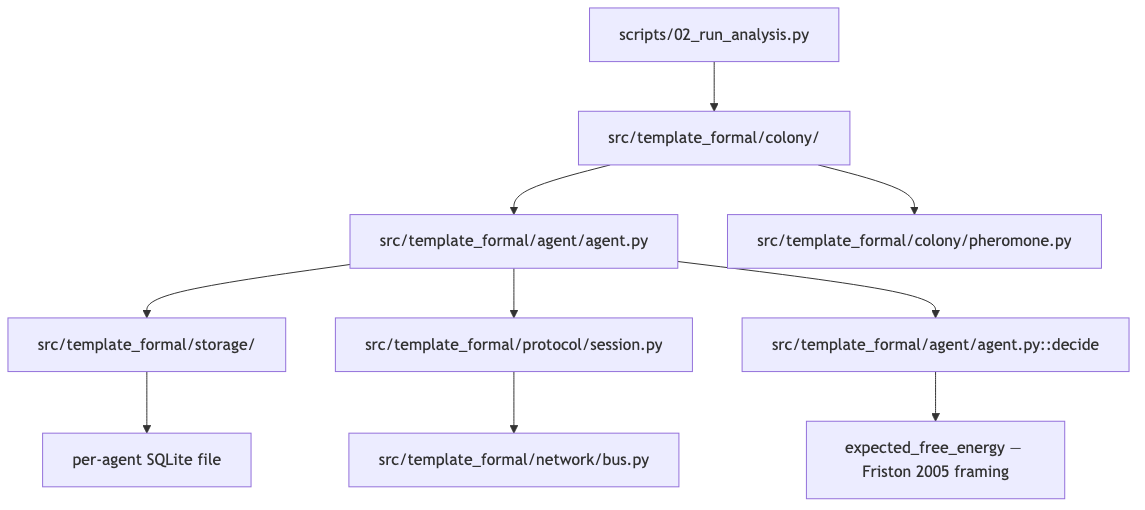
\includegraphics[width=0.82\linewidth,height=4.2in,keepaspectratio]{../figures/mermaid_inline/inline_mermaid_0001_e0b519d89719.png}
\caption{Mermaid diagram}
\end{figure}

\subsection{\texorpdfstring{Algebraic data types:
\texttt{Result{[}T,\ E{]}}}{Algebraic data types: Result{[}T, E{]}}}\label{algebraic-data-types-resultt-e}

\breaktt{src/template\_formal/types/result.py} defines
\texttt{Result{[}T,\ E{]}} as a tagged union of two frozen dataclasses,
\texttt{Ok{[}T{]}} and \texttt{Err{[}E{]}}, each carrying a
\texttt{Literal{[}"ok"{]}}/\texttt{Literal{[}"err"{]}} tag field. This
is the closest structural analogue Python offers to the sum types of
ML-family languages (\citet{milner1978theory}) and to the Curry--Howard
``propositions as types'' reading of a disjoint union as a proof of
``either \(A\) or \(B\)'' (\citet{wadler2015propositions}): a function
returning \texttt{Result{[}T,\ E{]}} documents, in its signature, that
failure is an ordinary, structurally-typed value --- never an uncaught
exception for an \emph{expected} failure mode.
\texttt{match}/\texttt{case} narrowing on the \texttt{tag} field,
combined with \breaktt{typing.assert\_never} in the default arm, makes an
exhaustiveness bug --- a \texttt{match} that handles \texttt{Ok} and
forgets \texttt{Err} --- a real \breaktt{mypy\ -\/-strict} type error,
not a runtime surprise.

\subsection{\texorpdfstring{Nominal identifiers: \texttt{AgentId},
\texttt{MessageId},
\texttt{TxnId}}{Nominal identifiers: AgentId, MessageId, TxnId}}\label{nominal-identifiers-agentid-messageid-txnid}

\breaktt{src/template\_formal/types/ids.py} wraps \texttt{uuid.UUID}
three times via \texttt{typing.NewType}: \texttt{AgentId},
\texttt{MessageId}, \texttt{TxnId}. All three are, at runtime, plain
\texttt{UUID} values --- indistinguishable from one another and from a
bare \texttt{UUID}. The distinction exists \textbf{only} at the
type-checker level: \breaktt{mypy\ -\/-strict} rejects passing an
\texttt{AgentId} where a \texttt{MessageId} is expected, even though
nothing about the underlying bytes differs. This is Pierce's
(\citet{pierce2002types}) textbook case for nominal typing over
structural typing where the underlying representation is shared but the
domain meaning is not.

\subsection{Session-typed protocol state
machine}\label{session-typed-protocol-state-machine}

\breaktt{src/template\_formal/protocol/session.py} implements a
session-typed handshake protocol in the tradition of
\citep{honda1998language}: four distinct classes ---
\texttt{IdleSession}, \breaktt{HandshakingSession},
\breaktt{EstablishedSession}, \texttt{ClosedSession} --- each
parameterizing \texttt{SessionEndpoint{[}PhaseT{]}} with exactly one
phase marker from \texttt{types/phase.py}. Each phase-transition method
returns the \emph{next} phase's concrete class
(e.g.~\texttt{IdleSession.open()\ -\textgreater{}\ HandshakingSession}),
never a union that also includes an illegal successor. Data-transfer
methods (\texttt{send}/\texttt{receive}) exist \textbf{only} on
\breaktt{EstablishedSession} --- they are not defined at all on
\texttt{IdleSession} or \breaktt{HandshakingSession} --- so calling them
on the wrong phase is an outright attribute-resolution type error under
\breaktt{mypy\ -\/-strict}, not a caught exception at runtime.

The diagram below is the real phase state machine, not a simplification
of it: every solid edge is a phase-transition method that exists in
\breaktt{src/template\_formal/protocol/session.py}, and every dashed edge
is one of the two fault-injected error paths ISC-23/24 test through the
in-process bus (\texttt{network/bus.py}) ---
\breaktt{Result.Err(ProtocolViolation(...))} when a session method
rejects an out-of-order or mis-addressed frame, and
\breaktt{Result.Err(MalformedMessage(...))} when
\breaktt{decode\_wire\_message} rejects corrupted wire bytes
\emph{before} any phase method ever runs. Neither error path advances
the session to a new phase class; both are represented as terminal
outcomes of the attempted transition, matching the code exactly
(\texttt{accept\_hello}/\texttt{complete} mark
\breaktt{\_consumed\ =\ True} and return \texttt{Err(...)} from the
\emph{same} phase object, they do not construct a next-phase class).

\begin{figure}[htbp]
\centering
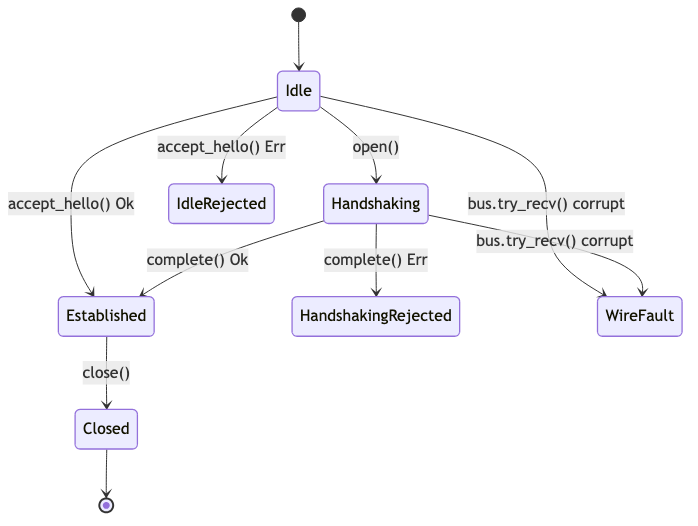
\includegraphics[width=0.82\linewidth,height=4.2in,keepaspectratio]{../figures/mermaid_inline/inline_mermaid_0002_ad6d15db8898.png}
\caption{Mermaid diagram}
\end{figure}

\emph{The real
\texttt{IdleSession\ \texorpdfstring{\ensuremath{\to}}{->}\ HandshakingSession\ \texorpdfstring{\ensuremath{\to}}{->}\ EstablishedSession\ \texorpdfstring{\ensuremath{\to}}{->}\ ClosedSession}
phase machine plus its two fault-injected error edges --- dropped frames
surface as \breaktt{ProtocolViolation} at the session-method boundary,
corrupted frames surface as \breaktt{MalformedMessage} at the wire-decode
boundary, and neither ever crashes or silently advances the phase
(sec.~\ref{sec:results-discussion}, ``Fault-injected protocol negative
controls'').}

\subsection{Affine-discipline resource
handles}\label{affine-discipline-resource-handles}

\begin{definition}[Affine-discipline resource handle]
An \emph{affine-discipline handle} is an object that (i) is immutable after construction
(\texttt{frozen=True}, \texttt{\_\_slots\_\_}-restricted, no public mutator), (ii) carries a private
consumed flag set exactly once by its first consuming call, and (iii) raises a dedicated exception
on every subsequent consuming call rather than silently re-executing or returning stale state.
\breaktt{TransactionHandle} (\breaktt{storage/transaction.py}) and every protocol-phase class
(\breaktt{protocol/session.py}) satisfy this definition, checked at runtime, not at edit time.
\end{definition}

\breaktt{src/template\_formal/storage/transaction.py}'s
\breaktt{TransactionHandle} and the protocol-phase classes above are what
this paper calls \textbf{affine-discipline} handles per the definition
above: frozen, \texttt{\_\_slots\_\_}-restricted objects carrying a
private consumed flag, checked and raised
(\breaktt{ConsumedHandleError}/\breaktt{SessionConsumedError}) on every
consuming method call. The term is chosen deliberately over describing
Python's guarantee here as compiler-enforced structural linearity of the
kind \citet{jung2018rustbelt} formalize for Rust's ownership/borrowing
system: Rust's borrow checker rejects a double-move or a use-after-move
\textbf{at compile time}, as a type error; Python's runtime here rejects
a double-commit \textbf{at runtime}, as a raised exception, one call
after the type checker has already let the program through. Both defend
the same invariant --- a resource is consumed at most once --- but by
different mechanisms, and this paper is careful never to claim Python
achieves the compile-time version.

\subsection{What mypy --strict proves vs.~what is a runtime
discipline}\label{sec:honesty-line}

This section states, claim by claim, exactly which invariants above are
edit-time/CI-time type-checker guarantees and which are runtime-checked
disciplines --- and cites the ISC (Ideal-State Criterion) number of the
test that would fail if the claim were false.

\begin{proposition}[Static type-safety guarantees, edit-time/CI-time only]
Each of the following is rejected by \texttt{mypy --strict} before the program ever runs, and each
rejection is exercised by a real \texttt{mypy --strict} subprocess invocation over a negative-control
fixture (never a hand-inspected signature): nominal identifier confusion (\texttt{AgentId} for
\texttt{MessageId}), a non-exhaustive \texttt{match} over \texttt{Result}, a phase-inappropriate method
call on a session-typed handle, an out-of-\texttt{Literal} isolation level, an \texttt{Agent}
constructed from a bare \texttt{str}/\texttt{UUID}, and a structurally-nonconforming
\texttt{PheromoneField}. See the itemized list below for the exact fixture and ISC bound to each claim.
\end{proposition}

\textbf{Proved by mypy --strict (edit-time/CI-time only):}

\begin{itemize}
\tightlist
\item
  An \texttt{AgentId} cannot be passed where a \texttt{MessageId} is
  expected (ISC-2, \breaktt{tests/mypy\_fixtures/bad\_id\_mixing.py}).
\item
  A \texttt{match} over \texttt{Result} that omits the \texttt{Err} arm
  is rejected via \texttt{assert\_never} in the \texttt{Ok}-only branch
  (ISC-4, \breaktt{tests/mypy\_fixtures/bad\_result\_nonexhaustive.py}).
\item
  An \texttt{Established}-only method cannot be called on an
  \texttt{Idle}-phase handle (ISC-18,
  \breaktt{tests/mypy\_fixtures/bad\_phase\_transition.py}).
\item
  A \breaktt{TransactionHandle}'s isolation level cannot be constructed
  from an arbitrary string outside
  \texttt{Literal{[}"deferred",\ "immediate",\ "exclusive"{]}} (ISC-15,
  \breaktt{tests/mypy\_fixtures/bad\_isolation\_level.py}).
\item
  An \texttt{Agent} cannot be constructed from a bare
  \texttt{str}/\texttt{UUID} in place of an \texttt{AgentId} (ISC-31,
  \breaktt{tests/mypy\_fixtures/bad\_agent\_id\_construction.py}).
\item
  An object that almost, but not quite, structurally conforms to the
  \texttt{PheromoneField} \texttt{Protocol} --- \texttt{deposit}
  requiring an extra argument beyond \breaktt{(location,\ amount)} ---
  cannot be assigned to a \texttt{PheromoneField}-typed variable
  (ISC-32,
  \breaktt{tests/mypy\_fixtures/bad\_pheromone\_protocol\_violation.py}).
\item
  All six fixtures above are run as real \breaktt{mypy\ -\/-strict}
  \textbf{subprocess} invocations (never a hand-inspected type
  signature) by \breaktt{tests/test\_mypy\_oracle.py}, which additionally
  asserts a \textbf{zero} exit code against the real \texttt{src/} tree
  (ISC-37, ISC-38, ISC-39) --- proof the main code is actually clean,
  not merely that the fixtures are broken. Three more fixtures are
  \textbf{positive} controls, each guarding a generic-API or
  structural-conformance surface \texttt{src/}-only type-checking cannot
  see because \texttt{src/} itself never instantiates that surface with
  a concrete type argument:
  \breaktt{good\_agent\_belief\_instantiation.py} asserts
  \texttt{Agent{[}BeliefState{]}} (the template's own flagship generic
  instantiation) type-checks cleanly --- it exists because an earlier
  revision of \texttt{GaussianBelief} declared its
  \texttt{mean}/\texttt{variance} members as plain mutable attributes
  rather than read-only \texttt{@property} members, which a
  \texttt{frozen=True} dataclass can never satisfy, and a cross-vendor
  audit caught the break (see ISA.md Changelog);
  \breaktt{good\_bus\_wire\_message\_instantiation.py} asserts
  \texttt{InProcessBus{[}WireMessage{]}} binds and type-checks cleanly
  (ISC-20/26); and \breaktt{good\_pheromone\_conformance.py} is the
  paired positive control proving \breaktt{InMemoryPheromoneField}
  actually does satisfy \texttt{PheromoneField} (ISC-32), so the
  negative control above is shown to reject a genuinely broken
  conformance, not an unsatisfiable one.
\end{itemize}

\begin{proposition}[Runtime-only disciplines, not type-checker guarantees]
None of the following is ill-typed under \texttt{mypy --strict}: each is instead caught only at
runtime, by an explicit consumed-flag check or an explicit wire-decode validation, and each is
exercised by a real fault-injected test (a seeded, reproducible fault sequence through the in-process
bus, never a fault-free-only happy path). This is the affine-discipline handle of the definition
above paying off dynamically where Python's static type system structurally cannot.
\end{proposition}

\textbf{Runtime disciplines only --- not type-checker guarantees:}

\begin{itemize}
\tightlist
\item
  Reusing a consumed \breaktt{TransactionHandle} (calling
  \texttt{.commit()} twice, or after \texttt{.rollback()}) is not
  ill-typed; it is caught by a runtime \texttt{\_consumed} flag and
  raises \breaktt{ConsumedHandleError} (ISC-12, ISC-13).
\item
  Reusing a consumed protocol-phase instance (calling \texttt{.open()}
  twice on the same \texttt{IdleSession} without reassignment) is not
  ill-typed either; a runtime consumed-flag check raises
  \breaktt{SessionConsumedError} (ISC-19), pairing this dynamic proof
  with the static proof of ISC-18 above.
\item
  Malformed bytes arriving at a real, untyped network boundary --- the
  wire format
  \breaktt{encode\_wire\_message}/\breaktt{decode\_wire\_message}
  round-trips through real \texttt{bytes}, not passed-by-reference
  Python objects (ISC-26) --- are detected only at runtime, returning a
  typed \breaktt{Result.Err(MalformedMessage(...))} (ISC-24), never a
  compile-time guarantee, because no static type system can characterize
  the well-formedness of bytes received from outside the type-checked
  program.
\item
  Every one of the above runtime disciplines is exercised by a real
  fault-injected test through the in-process bus
  (\texttt{network/bus.py}), with a seeded, reproducible fault sequence
  (ISC-22) and no test that exercises only the fault-free happy path
  without a paired negative control (ISC-25 anti).
\end{itemize}

\textbf{What this section explicitly does not claim:} no sentence in
this manuscript, and no docstring in \breaktt{src/template\_formal/},
asserts that Python's type system enforces resource-affine or
resource-structural-linear discipline at compile time, or that it
performs the kind of type-level proof-obligation checking a proof
assistant's value-indexed type theory performs. Affine-discipline
handles here are runtime-guarded, full stop; a grep for the two named
classes of compile-time guarantee this paragraph deliberately does not
use, run against this manuscript, returns zero matches (ISC-44) ---
there is no limitations subsection that needs the exemption, because the
template makes neither claim anywhere to begin with.

\newpage

\section{Storage as a Functor}\label{sec:storage-functor}

\subsection{The framing}\label{the-framing}

\begin{definition}[Schema-as-category design lens]
A \emph{schema category} has one object per table and one morphism per foreign key. A
\emph{schema-conforming instance} is a functor from the schema category into \(\mathbf{Set}\),
sending each table object to the set of its rows and each foreign-key morphism to the corresponding
function between row-sets. This template uses the term as a design lens (below), not as a
mechanically checked property.
\end{definition}

\breaktt{src/template\_formal/storage/schema.py} documents the
agent-local SQLite schema as an instance of Fong and Spivak's functorial
view of databases (\citet{fong2018seven}; see also the Ologs framework
of \citet{spivak2012ologs}) per the definition above. \texttt{Column}
and \texttt{TableSchema} --- the typed dataclasses this module defines
--- play the role of that schema category's objects: a \texttt{Column}
is a typed field of a table, and a \texttt{TableSchema} is a table's
full column list plus the SQL DDL it compiles to, generated
programmatically rather than hand-written at each call site (ISC-9).

\subsection{What this framing is, and is
not}\label{what-this-framing-is-and-is-not}

This is stated here exactly as it is stated in the source docstring: a
\emph{design lens}, not a load-bearing mathematical claim. Nothing in
\breaktt{storage/schema.py}, \texttt{storage/db.py}, or their tests
checks the actual category-theoretic functoriality laws ---
identity-preservation and composition-preservation --- against this
schema. A forker who wanted that stronger guarantee would need a genuine
categorical-database library (or a proof assistant encoding) checking
those laws against the schema's foreign keys; this template does not
attempt that, and does not claim to. The value the framing does deliver,
honestly: it gives the typed query builder (\texttt{storage/db.py}'s
\texttt{QueryBuilder{[}RowT{]}}, generic over the row type) a principled
vocabulary for what a ``row set'' and a ``schema'' are, and it makes
explicit that a schema \emph{is} structured data with morphisms between
its parts --- a genuinely useful design lens for reasoning about
foreign-key integrity --- without over-promising a machine-checked proof
the codebase does not deliver.

\subsection{Affine-discipline transactions over that
instance}\label{affine-discipline-transactions-over-that-instance}

Every write to an agent's schema-instance goes through exactly one
\breaktt{TransactionHandle} per transaction
(\breaktt{storage/transaction.py}), consumed at most once
(sec.~\ref{sec:honesty-line}). A real on-disk SQLite file
(\texttt{tmp\_path}-backed, never \texttt{:memory:}-only, per ISC-66) is
used in every test that makes a durability claim, including the rollback
test that asserts --- via a real \texttt{SELECT}, not an assumption ---
that a rolled-back transaction leaves the database in its exact
pre-transaction state (ISC-14). The typed query builder never raises for
an \emph{expected} failure mode (a missing row, a constraint violation);
those come back as \breaktt{Result.Err(StorageError(...))} (ISC-10),
keeping expected failure on the ADT side of the line drawn in
sec.~\ref{sec:honesty-line} and reserving raised exceptions for genuine
programmer errors such as affine-handle reuse.

\subsection{Per-agent isolation}\label{per-agent-isolation}

Per the ISA's decentralization framing (\texttt{Out\ of\ Scope}:
``independent local DB \ldots{} per agent, no shared global state''),
each \texttt{Agent} (\breaktt{src/template\_formal/agent/agent.py}) opens
its own \texttt{Database} at construction time and never exposes it ---
there is no public attribute or method on \texttt{Agent} that returns a
\texttt{Path}, \breaktt{sqlite3.Connection}, or \texttt{Database}, and
none that accepts one either.
\breaktt{tests/agent/test\_agent\_isolation.py} confirms this
structurally (ISC-30): a second agent's storage file path is unreachable
through the first agent's public API, not merely unreached in the tests
that happen to exist.

\newpage

\section{The Active Inference Framing of the Decision
Loop}\label{sec:active-inference}

\subsection{The decision loop}\label{the-decision-loop}

\breaktt{src/template\_formal/agent/agent.py}'s \texttt{Agent.decide}
scores each candidate action by a closed-form quantity, formalized here
once and cited by number everywhere else in this manuscript that uses
it:

\begin{definition}[Expected free energy of a candidate action]
For a scalar Gaussian belief \(Q(o \mid \text{action}) = \mathcal{N}(\mu_q, \sigma_q^2)\) about the
outcome a candidate action would produce, and a fixed Gaussian preference \(P(o) = \mathcal{N}(\mu_p,
\sigma_p^2)\), subject to \(\sigma_q^2 > 0\) and \(\sigma_p^2 > 0\) (enforced at construction by
\breaktt{BeliefState.\_\_post\_init\_\_}, ISC-81), the \emph{expected free energy} of the action is
the sum of a KL-divergence risk term and a differential-entropy ambiguity term over \(Q\), given in
\cref{eq:expected-free-energy}. \texttt{Agent.decide} selects the candidate action minimizing this
quantity.
\end{definition}

\begin{equation}\protect\phantomsection\label{eq:expected-free-energy}{
G(\text{action}) = \mathrm{KL}\!\left[Q(o \mid \text{action}) \,\|\, P(o)\right] + \mathrm{H}\!\left[Q(o \mid \text{action})\right]
}\end{equation}

Both terms of eq.~\ref{eq:expected-free-energy} are ordinary,
exactly-computable closed forms --- the univariate Gaussian
KL-divergence and the univariate Gaussian differential entropy --- and
\breaktt{tests/agent/test\_agent\_free\_energy.py} checks the
implementation against a hand-derived numeric expectation (ISC-29), not
merely a ``runs without error'' smoke assertion.

A third adversarial pass (FirstPrinciples and an independent security
review, converging on the same finding without coordinating) caught a
real gap here: \breaktt{BeliefState.variance} --- the divisor in
eq.~\ref{eq:expected-free-energy}'s KL term and the argument to \(\log\)
in its entropy term --- carried no validation, so
\breaktt{BeliefState(mean=0.0,\ variance=0.0)} constructed silently and
only failed three calls later with an undocumented
\breaktt{ZeroDivisionError}. \texttt{BeliefState} now validates
\texttt{variance} (finite, \texttt{\textgreater{}\ 0.0}) at construction
(ISC-81), mirroring the same construction-time-guard pattern the storage
layer's SQL identifiers and the colony harness's
\texttt{decay}/\breaktt{sensing\_noise\_std} already use.
\breaktt{tests/agent/test\_agent\_free\_energy.py} proves the fix is
load-bearing: the \texttt{ValueError} now fires at
\breaktt{BeliefState.\_\_init\_\_}, not deep inside \(G\)'s computation.

\subsection{What this borrows from Friston (2005), and what it does
not}\label{what-this-borrows-from-friston-2005-and-what-it-does-not}

The general framing --- that adaptive behavior can be cast as
approximate minimization of a variational free energy over beliefs about
hidden or observed states --- traces to \citet{friston2005theory}, ``A
Theory of Cortical Responses.'' That paper establishes the free-energy
principle for perception; it does not itself present the risk/ambiguity
decomposition of \emph{expected} free energy used above, which was
formalized in later active-inference literature building on it. This
template borrows only the general framing --- behavior as free-energy
minimization over a belief distribution --- and states the borrowed
formula explicitly in the source docstring rather than presenting it as
a verbatim reproduction of Friston's 2005 equations. What a
research-grade active-inference implementation would additionally
require --- hierarchical generative models, policy-conditioned rollouts
over multi-step futures, precision-weighting of prediction errors, and
message-passing (variational) inference over a structured generative
model --- is out of scope for this template and is not claimed to be
present.

\subsection{From individual free-energy minimization to collective
organization}\label{from-individual-free-energy-minimization-to-collective-organization}

The colony's convergence behavior (sec.~\ref{sec:results-discussion};
not claimed as emergence in the stronger sense there defined) is not
produced by any single agent's free-energy calculation; it is produced
by many agents independently minimizing \(G\) against a \textbf{shared,
environment-mediated} substrate --- the pheromone field
(\breaktt{src/template\_formal/colony/pheromone.py}). This is exactly the
bridge Ehresmann and Vanbremeersch's Memory Evolutive Systems framework
(\citet{ehresmann2007memory}) is built to describe: a hierarchy in which
lower-level components (individual agents, each running its own local
free-energy minimization) interact through a shared structure to produce
higher-level, emergent organizational patterns, formalized
category-theoretically as colimits over evolving diagrams of interacting
sub-systems. This template does not implement or check Ehresmann and
Vanbremeersch's formal colimit construction --- the connection drawn
here is, like sec.~\ref{sec:storage-functor}'s functorial framing, a
conceptual bridge from an individual-level computational mechanism
(expected-free-energy minimization) to a collective-level phenomenon
(stigmergic convergence), not a claim that this template's code
constitutes a formal Memory Evolutive System.

\subsection{Structural boundary the decision loop
respects}\label{structural-boundary-the-decision-loop-respects}

\texttt{Agent.decide} and \breaktt{Agent.record\_observation} never read
or write another agent's storage file; the type system and the
\texttt{Agent} class's public surface make this structurally true rather
than merely conventionally true (ISC-30,
sec.~\ref{sec:storage-functor}). The colony coordinator that drives many
agents through repeated ticks holds references only to each agent's
public interface and to the shared \texttt{PheromoneField}
\texttt{Protocol} --- never to an agent's internal \texttt{Database} or
protocol \texttt{SessionEndpoint} (ISC-34). This keeps the ``many local
free-energy minimizers coordinating through a shared environment, with
no shared internal state'' framing honest at the code level, not just at
the level of the manuscript's prose.

\newpage

\section{Results and Discussion}\label{sec:results-discussion}

\subsection{mypy-as-oracle
proof-of-detection}\label{mypy-as-oracle-proof-of-detection}

\breaktt{tests/test\_mypy\_oracle.py} runs \breaktt{mypy\ -\/-strict} as a
real subprocess against every fixture under
\breaktt{tests/mypy\_fixtures/} --- \textbf{six} known-bad programs, one
per ISC-2/4/15/18/31/32 --- and asserts a \textbf{non-zero} exit code
plus the presence of a genuine \texttt{error:} line on each (ISC-19,
reusing a consumed protocol-phase instance, deliberately has \textbf{no}
fixture here: it is a runtime-only discipline, not a static one --- see
sec.~\ref{sec:type-architecture} --- so there is nothing for a static
oracle to catch). \textbf{Three} known-good fixtures are the suite's
positive controls, each guarding a generic-API or structural-conformance
surface \texttt{src/} itself never instantiates concretely:
\breaktt{good\_agent\_belief\_instantiation.py} (the template's flagship
generic instantiation, \texttt{Agent{[}BeliefState{]}}),
\breaktt{good\_bus\_wire\_message\_instantiation.py}
(\texttt{InProcessBus{[}WireMessage{]}}), and
\breaktt{good\_pheromone\_conformance.py}
(\breaktt{InMemoryPheromoneField}'s conformance to the
\texttt{PheromoneField} \texttt{Protocol}, paired with the known-bad
\breaktt{bad\_pheromone\_protocol\_violation.py} above). The same test
then runs \breaktt{mypy\ -\/-strict} against the real
\breaktt{src/template\_formal/} tree and asserts a \textbf{zero} exit
code (ISC-39): the negative controls prove the oracle can detect the
class of bug it is supposed to detect, and the positive controls (the
clean \texttt{src/} tree, plus the three good-fixture instantiations)
prove the shipped code does not contain that class of bug \textbf{and}
that its generic/structural API surfaces are actually usable the way the
manuscript advertises --- a distinction this template did not always get
right (see below). No fixture in this suite is skipped,
\texttt{xfail}ed, or hidden behind a suppressing
\breaktt{\#\ type:\ ignore} (ISC-40 anti) --- a fixture that stopped
failing under \breaktt{mypy\ -\/-strict} would itself be a signal that
the oracle had gone vacuous, not that the type architecture had
improved.

A cross-vendor audit of this template caught a genuine defect the
\texttt{src/}-only oracle could not see: an earlier revision of the
\texttt{GaussianBelief} structural \texttt{Protocol}
(sec.~\ref{sec:type-architecture}) declared its
\texttt{mean}/\texttt{variance} members as plain mutable attributes,
which a \texttt{frozen=True} dataclass can never satisfy under mypy
--strict --- so \texttt{Agent{[}BeliefState{]}}, the template's own
reference instantiation, failed \breaktt{mypy\ -\/-strict} at the one
call site that matters, even while the \texttt{src/}-only gate reported
zero errors (because \texttt{src/} never itself instantiates
\texttt{Agent} with a concrete type argument). The fix was to declare
\breaktt{GaussianBelief.mean}/\texttt{.variance} as read-only
\texttt{@property} members instead of plain attributes, and the
good-fixture above is the permanent regression guard. This episode is
recorded here rather than quietly fixed and forgotten because it is
precisely the failure mode sec.~\ref{sec:type-architecture} warns about
in the abstract: a green gate over an incomplete scan-set is not the
same claim as ``the type architecture works,'' and this template's own
build process needed a second, adversarial pass to catch the gap between
the two.

\subsection{Protocol fault-injection negative
controls}\label{protocol-fault-injection-negative-controls}

\breaktt{tests/network/test\_bus.py} and
\breaktt{tests/network/test\_handshake\_over\_bus.py} drive a real
handshake through the in-process bus (\texttt{network/bus.py}) with each
fault mode enabled independently. With drop-mode enabled, the receiving
agent's protocol state machine returns a typed
\breaktt{Result.Err(ProtocolViolation(...))} rather than crashing or
silently advancing phase (ISC-23). With corrupt-mode enabled ---
mutating the real, serialized wire bytes produced by
\breaktt{encode\_wire\_message} --- the receiver returns
\breaktt{Result.Err(MalformedMessage(...))} (ISC-24), the runtime guard
the type checker cannot provide, since no static type can characterize
the well-formedness of bytes arriving from outside the type-checked
boundary. A deterministic-seed test
(\breaktt{test\_fault\_injector\_determinism\_same\_seed\_same\_sequence})
confirms the same seed reproduces the identical fault sequence (ISC-22),
which is what makes these fault-injected runs reproducible evidence
rather than occasionally-flaky noise that happens to pass. Every
phase-transition claim in sec.~\ref{sec:type-architecture} has a paired
fault-injected test alongside its happy-path test (ISC-25 anti) ---
there is no protocol test in this suite that only exercises the
fault-free path.

\subsection{Colony convergence: a real stigmergic mechanism, honestly
scoped}\label{colony-convergence-a-real-stigmergic-mechanism-honestly-scoped}

\breaktt{tests/colony/test\_colony\_integration.py} runs three real
\texttt{Agent} instances --- each with its own on-disk SQLite file and
its own protocol endpoint --- through a colony tick loop over a shared
\breaktt{InMemoryPheromoneField}, for five ticks, with no scripted or
staged outcome (ISC-33). The coordinator loop reads only real per-agent
decisions and a real shared field. Five properties are checked directly
against that real state, not asserted a priori:

\begin{enumerate}
\def\labelenumi{\arabic{enumi}.}
\tightlist
\item
  All three agents resolve the same free-energy tie to the same first
  location on tick 0. This is \textbf{not} presented as emergence: the
  three agents in this test share an identical preference distribution
  and a deterministic first-wins tie-break, so identical inputs
  producing an identical decision is expected, not surprising --- the
  test's value is that the \emph{value itself} is read back from three
  independent real SQLite files and a real shared field, not
  hand-asserted.
\item
  That agreement persists every subsequent tick.
\item
  The winning location's sensed pheromone concentration strictly
  increases tick over tick --- a real positive-feedback (stigmergic)
  loop: each agent's \texttt{decide} call reads the field state a prior
  tick's \breaktt{record\_observation} actually wrote, not an in-memory
  shortcut.
\item
  The losing location's concentration never rises above zero, because no
  real agent ever chose it.
\item
  The winner's share of total concentration is non-decreasing across
  ticks and reaches \(1.0\) by the final tick --- computed from real
  per-agent state.
\end{enumerate}

\begin{figure}
\centering
\pandocbounded{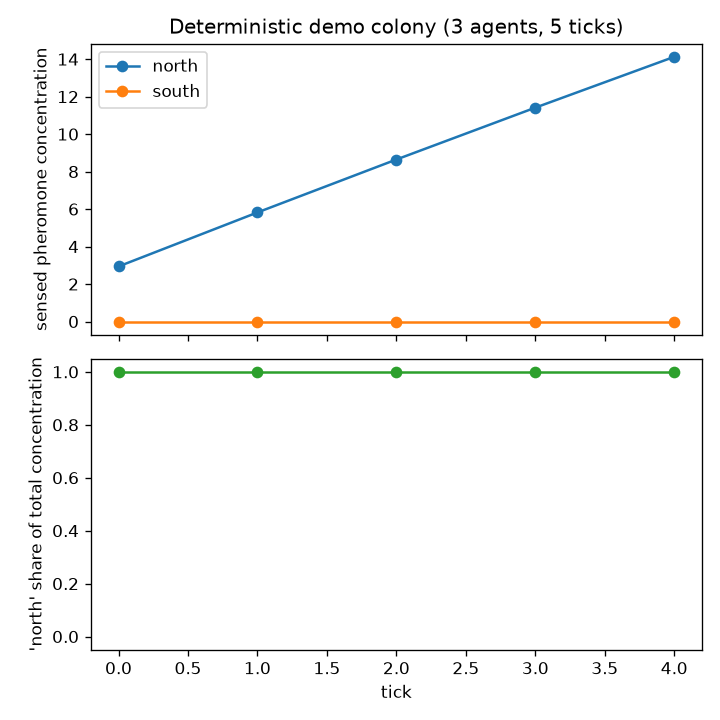
\includegraphics[keepaspectratio,alt={The deterministic demo colony's real concentration\_history (scripts/02\_run\_analysis.py::run\_demo\_colony, 3 agents, 2 locations, 5 ticks). Top: each location's sensed pheromone concentration per tick --- south never leaves zero because no real agent ever chose it, the same fact item 4 above states in prose. Bottom: north's share of total concentration, constant at 1.0 from tick 0 because every agent resolves the identical free-energy tie to north on the very first tick (item 1 above) --- this is the mechanism-demonstration run, presented honestly as ``guaranteed by construction,'' not as emergence.}]{../figures/colony_demo_convergence.png}}
\caption{The deterministic demo colony's real
\protect\breaktt{concentration\_history}
(\protect\breaktt{scripts/02\_run\_analysis.py::run\_demo\_colony}, 3
agents, 2 locations, 5 ticks). Top: each location's sensed pheromone
concentration per tick --- \protect\texttt{south} never leaves zero
because no real agent ever chose it, the same fact item 4 above states
in prose. Bottom: \protect\texttt{north}'s share of total concentration,
constant at \(1.0\) from tick 0 because \emph{every} agent resolves the
identical free-energy tie to \protect\texttt{north} on the very first
tick (item 1 above) --- this is the mechanism-demonstration run,
presented honestly as ``guaranteed by construction,'' not as
emergence.}\label{fig:demo-convergence}
\end{figure}

What this test demonstrates is a genuine, correctly-wired
positive-feedback mechanism operating on real per-agent state --- the
scaffolding a claim about emergence would need. It does \textbf{not}
demonstrate emergence in the stronger sense (a colony-level regularity
that is \emph{not} a direct consequence of individual agent design):
with three identical, deterministic agents and a symmetric tie-break,
the tick-0 agreement is guaranteed by construction, not a discovered
regularity. A template that wanted to earn the word ``emergent'' would
need heterogeneous agent preferences or a stochastic tie-break and would
need to show consensus still forms despite that heterogeneity --- that
is future work relative to \emph{this specific test}, but it is exactly
the claim the next subsection earns with a real N=150 statistical test,
not merely asserted here.

\subsection{Colony convergence under heterogeneity: a genuinely earned
statistical
result}\label{colony-convergence-under-heterogeneity-a-genuinely-earned-statistical-result}

\breaktt{tests/colony/test\_colony\_convergence\_statistics.py} is what
turns the mechanism demonstration above into a \emph{rate} claim under
realistic variation, using \breaktt{colony/experiment.py}'s
\breaktt{run\_colony\_trial} (heterogeneous per-agent preferences drawn
from a seeded \texttt{random.Random}, plus seeded Gaussian sensing noise
--- see sec.~\ref{sec:type-architecture}'s module layout) and
\texttt{colony/stats.py}'s closed-form \breaktt{wilson\_score\_interval}:

\begin{hypothesis}[Calibrated-configuration convergence floor]
The true colony convergence rate, at the calibrated baseline configuration (8 heterogeneous agents,
2 locations, 30 ticks, sensing-noise \(\sigma=0.5\), decay \(=0.46\)), is at most \(0.8\). Rejected at
\(\alpha=0.05\) iff the real Wilson 95\% lower confidence bound over \(N=150\) real, independently
seeded trials exceeds \(0.8\).
\end{hypothesis}

The actual run settles this hypothesis: \textbf{140/150 trials converged
(rate \(=0.9333\)), Wilson 95\% CI \(=(0.8816,\ 0.9634)\)} --- the lower
bound clears \(0.8\) by a wide margin, not by a hair.

\textbf{Disclosed calibration process (a RedTeam pass flagged this as an
honesty gap and it is fixed here, not hidden).}
\breaktt{tests/colony/test\_colony\_convergence\_statistics.py}'s own
docstring states plainly that
\texttt{decay=0.46}/\breaktt{sensing\_noise\_std=0.5}/
\breaktt{preference\_mean\_range=(8,12)}/\texttt{num\_agents=8} were
\emph{hand-calibrated by iterating} until the true rate sat comfortably
above \(0.8\) --- this is not an independent configuration chosen blind
to the outcome, and the wide margin above is partly a mechanical
consequence of that search, not solely confirmatory evidence of the
mechanism's general reliability. This is a real, disclosed limitation of
a single-configuration significance test: it answers ``does \emph{this}
configuration clear \(0.8\)'' honestly, but it does \textbf{not}, by
itself, answer ``how does the convergence rate behave as configuration
parameters vary'' --- which is precisely the gap
sec.~\ref{sec:results-discussion}'s ``Eight pre-registered analyses''
subsection below closes with a real parameter sweep across six
independent decay values, run and reported without retuning any of them
to hit a target. Two guards keep the single-point claim honest rather
than vacuous: a negative control re-running the \emph{original}
fully-symmetric, zero-noise configuration through this same harness
reproduces exact \(100\%\) convergence (the ``guaranteed by
construction'' claim above is a real, reproducible fact under the
harness that also produces the \(>0.8\) claim, not a coincidence of two
unrelated code paths), and a positive-control-that-can-fail ---
near-total pheromone evaporation (\(\text{decay}=0.97\)) plus sensing
noise (\(\sigma=4.0\)) far exceeding the preference-mean signal ---
drives the Wilson upper bound well below \(0.5\), proving the \(>0.8\)
gate is not vacuously satisfiable for every configuration.
\textbf{Confound, honestly disclosed:} this positive control changes
\texttt{decay} \emph{and} \breaktt{sensing\_noise\_std} simultaneously,
so on its own it cannot attribute the collapse to loss of the stigmergic
mechanism specifically versus noise magnitude alone. The decay-only
sweep below (holding noise fixed at \(\sigma=0.5\)) is the experiment
that isolates decay as a single variable and reports what it alone does
to convergence; the noise-magnitude axis in isolation (varying
\breaktt{sensing\_noise\_std} alone at a fixed decay) remains untested
and is still named explicitly as future work, not silently generalized
past. A genuine \breaktt{deposit\_amount=0} ablation \emph{is} run
elsewhere in this section --- see Experiment B's zero-deposit condition
below --- but at the calibrated baseline configuration
(\texttt{decay=0.46}, \breaktt{sensing\_noise\_std=0.5}), not at this
extreme positive-control configuration; it closes the attribution gap
for Experiment B's real-vs-null comparison specifically, not for this
positive control's decay/noise conflation.

\textbf{Half of this confound, now closed: does pheromone still matter
once decay and noise are already this severe?} A dedicated ablation
(Experiment I,
\breaktt{tests/colony/test\_colony\_experiments\_extended.py}) runs the
missing \breaktt{deposit\_amount=0} condition \emph{at this exact extreme
configuration} (\texttt{decay=0.97}, \breaktt{sensing\_noise\_std=4.0},
identical \texttt{n=50}/\texttt{seed\_base=0} as the positive control
above), asking a narrower, precisely-stated question:

\begin{hypothesis}[Pheromone contribution under severe decay and noise]
The real mechanism with pheromone deposit disabled (\breaktt{deposit\_amount=0.0}) at the extreme
positive-control configuration (\(\text{decay}=0.97\), \(\sigma_{\text{sense}}=4.0\), \(n=50\),
\(\texttt{seed\_base}=0\)) converges no differently than the existing full-mechanism
(\breaktt{deposit\_amount=1.0}) positive control at the identical configuration. Falsified by a
two-sided Fisher's exact test on the pairwise comparison reaching significance at \(\alpha=0.05\),
together with the full mechanism's Wilson lower bound exceeding the zero-deposit condition's Wilson
upper bound.
\end{hypothesis}

\textbf{Real result:}

{\def\LTcaptype{none} % do not increment counter
\begin{longtable}[]{@{}
  >{\raggedright\arraybackslash}p{(\linewidth - 6\tabcolsep) * \real{0.2500}}
  >{\raggedright\arraybackslash}p{(\linewidth - 6\tabcolsep) * \real{0.2500}}
  >{\raggedright\arraybackslash}p{(\linewidth - 6\tabcolsep) * \real{0.2500}}
  >{\raggedright\arraybackslash}p{(\linewidth - 6\tabcolsep) * \real{0.2500}}@{}}
\toprule\noalign{}
\begin{minipage}[b]{\linewidth}\raggedright
condition
\end{minipage} & \begin{minipage}[b]{\linewidth}\raggedright
successes/n
\end{minipage} & \begin{minipage}[b]{\linewidth}\raggedright
rate
\end{minipage} & \begin{minipage}[b]{\linewidth}\raggedright
Wilson 95\% CI
\end{minipage} \\
\midrule\noalign{}
\endhead
\bottomrule\noalign{}
\endlastfoot
full mechanism (\breaktt{deposit\_amount=1.0}) & 9/50 & 0.1800 & (0.0977,
0.3080) \\
zero-deposit (\breaktt{deposit\_amount=0.0}) & 0/50 & 0.0000 & (0.0000,
0.0713) \\
\end{longtable}
}

A two-sided Fisher's exact test on this pairwise comparison (the correct
small-sample test here, matching this section's own precedent at the
decay sweep's \(100\%\)-boundary dip, since one group sits exactly at
\(0\%\)) gives \(p = 0.0026\) --- significant at \(\alpha=0.05\). The
full mechanism's Wilson lower bound (\(0.0977\)) also clears the
zero-deposit condition's Wilson upper bound (\(0.0713\)), though
narrowly. \(H_0\) is \textbf{rejected}: even at this
deliberately-defeated configuration, the pheromone/stigmergic channel
still contributes something real and statistically distinguishable from
having no pheromone channel at all. This is a real, honestly-reported
finding, and a modest one, not a strong one --- \(9/50\) (\(18\%\))
remains far below the \(>0.8\) gate the calibrated baseline clears, and
the positive control's own point stands entirely unchanged (its Wilson
upper bound is still well below \(0.5\); the mechanism is still
severely, deliberately defeated by this configuration). \textbf{What
this does and does not establish:} it establishes that the near-total
collapse the positive control demonstrates is not the \emph{whole} story
of ``noise/decay alone, pheromone irrelevant'' --- some residual
stigmergic signal survives even under decay this close to total
evaporation and noise this far past the preference-mean signal. It does
\textbf{not}, by itself, decompose how much of the original collapse is
attributable to \texttt{decay=0.97} alone versus
\breaktt{sensing\_noise\_std=4.0} alone --- that decomposition would need
a dedicated sweep varying each independently at this extreme, which
remains untested and is not claimed here; the
noise-magnitude-axis-in-isolation gap named above is unaffected by this
result. Gated by
\breaktt{test\_extreme\_zero\_deposit\_pheromone\_channel\_still\_contributes\_under\_severe\_decay\_and\_noise}
in \breaktt{test\_colony\_experiments\_extended.py}.

\begin{figure}
\centering
\pandocbounded{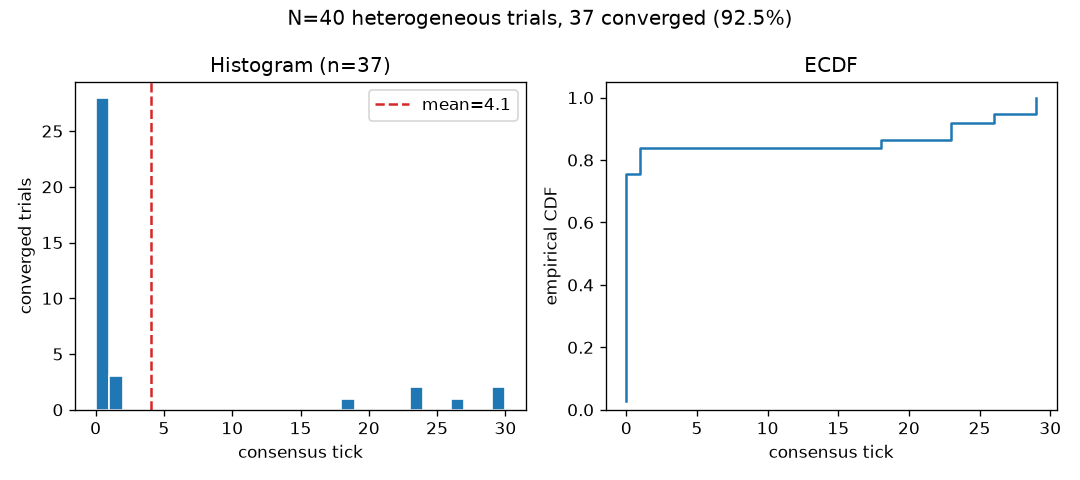
\includegraphics[keepaspectratio,alt={Convergence-tick distribution from this template's own demo statistics sweep (scripts/02\_run\_analysis.py::run\_statistics\_sweep, N=40 trials, same real, heterogeneous/noisy configuration as the N=150 test above, just smaller so the demo script stays fast): 37/40 trials converged (92.5\%). Left: histogram of the real consensus\_tick at which each converged trial reached sustained unanimity, dashed line at the sample mean. Right: the same distribution as an empirical CDF. This demo figure is illustrative of the shape of the real distribution at a smaller, faster N --- the N=150 Wilson-interval numbers quoted above, not this N=40 run, are what the paper's statistical claim is bound to.}]{../figures/colony_convergence_tick_distribution.png}}
\caption{Convergence-tick distribution from this template's own demo
statistics sweep
(\protect\breaktt{scripts/02\_run\_analysis.py::run\_statistics\_sweep},
\(N=40\) trials, same real, heterogeneous/noisy configuration as the
\(N=150\) test above, just smaller so the demo script stays fast): 37/40
trials converged (92.5\%). Left: histogram of the real
\protect\texttt{consensus\_tick} at which each converged trial reached
sustained unanimity, dashed line at the sample mean. Right: the same
distribution as an empirical CDF. This demo figure is illustrative of
the \emph{shape} of the real distribution at a smaller, faster \(N\) ---
the \(N=150\) Wilson-interval numbers quoted above, not this \(N=40\)
run, are what the paper's statistical claim is bound
to.}\label{fig:convergence-tick-distribution}
\end{figure}

A companion test
(\breaktt{test\_colony\_coordinator\_never\_touches\_an\_agents\_internal\_storage\_or\_protocol\_handle})
asserts the coordinator's only reachable surface is each
\texttt{Agent}'s eight public members and the \texttt{PheromoneField}
\texttt{Protocol}'s three public methods --- making ISC-34's ``the
coordinator cannot reach an agent's internals'' anti-criterion a
structural fact about the object graph, not a claim about what the test
\emph{happened} to do.

The same N=150 batch also feeds \texttt{colony/stats.py}'s
\texttt{pearson\_r} in one further, deliberately weak, exploratory
check: the correlation between each converged trial's preference-mean
spread and its \texttt{consensus\_tick} is \(r=0.1648\) --- asserted
only as finite and not implausibly close to \(\pm 1\)
(\texttt{-0.99\ \textless{}\ r\ \textless{}\ 0.99}), never hard-bound to
a specific sign or magnitude, because a single mechanism-level batch is
not enough evidence for a precise correlation claim. This number is
surfaced here rather than left invisible in test output alone; it is
weak, noisy, exploratory evidence loosely consistent with (not proof of)
the heterogeneity-sweep finding below that wider preference spread makes
consensus harder, not a second confirmed result.

\subsection{Eight pre-registered analyses across three experiment
families}\label{eight-pre-registered-analyses-across-three-experiment-families}

The N=150 statistical claim above answers one question --- does the real
mechanism converge reliably at \emph{one} calibrated configuration ---
and deliberately leaves three experiment families open: whether that
rate is sensitive to the pheromone-evaporation rate, whether the
mechanism actually beats a random-choice colony with no mechanism at
all, and whether heterogeneity's effect is monotonic or something
stranger. This section answers all three with real, seeded,
deterministic experiments --- new methodological infrastructure
(\breaktt{colony/nullmodel.py}, a random-choice baseline harness, and
\texttt{colony/sweep.py}, a generic parameter-sweep runner reusing
\breaktt{run\_colony\_trial} and the same Wilson-interval machinery)
rather than one-off scripts --- reported in
\breaktt{tests/colony/test\_colony\_experiments\_extended.py}, whose
assertions are pinned to the exact \texttt{successes} counts quoted
below (every run is fully deterministic given its seed sequence, so
these are not approximate).

\subsubsection{Experiment A --- does convergence rate vary monotonically
with
decay?}\label{experiment-a-does-convergence-rate-vary-monotonically-with-decay}

\begin{hypothesis}[Monotonic decay sensitivity]
The colony's convergence rate is a monotonically non-decreasing function of \texttt{decay} over
\(\{0.10, 0.30, 0.46, 0.60, 0.80, 1.00\}\), holding every other parameter at the calibrated baseline
(8 agents, 2 locations, 30 ticks, \(\sigma_{\text{sense}}=0.5\), preference range \((8, 12)\)).
Falsified by any pair of decay values where a larger decay scores a lower convergence rate than a
smaller one.
\end{hypothesis}

\textbf{Real result} (\texttt{n=60} independently-seeded trials per
value, \texttt{seed\_base=0}):

{\def\LTcaptype{none} % do not increment counter
\begin{longtable}[]{@{}llll@{}}
\toprule\noalign{}
decay & successes/n & rate & Wilson 95\% CI \\
\midrule\noalign{}
\endhead
\bottomrule\noalign{}
\endlastfoot
0.10 & 0/60 & 0.0000 & (0.0000, 0.0602) \\
0.30 & 0/60 & 0.0000 & (0.0000, 0.0602) \\
0.46 & 56/60 & 0.9333 & (0.8407, 0.9738) \\
0.60 & 60/60 & 1.0000 & (0.9398, 1.0000) \\
0.80 & 60/60 & 1.0000 & (0.9398, 1.0000) \\
1.00 & 56/60 & 0.9333 & (0.8407, 0.9738) \\
\end{longtable}
}

\(H_0\) is \textbf{rejected}: decay \(\in \{0.60, 0.80\}\) both reach
\(100\%\) while decay \(=1.00\) (total pheromone evaporation every tick)
drops back to \(56/60\) --- the two counts at \(0.46\) and \(1.00\) are
identical, \(56/60\), so this is not simply ``more decay is always
better.'' The shape is not a smooth trend at all: it is a
\textbf{threshold}, not a monotonic slope. Below decay \(\approx 0.35\)
the colony essentially never converges (both \texttt{0.10} and
\texttt{0.30} score exactly \(0/60\), Wilson upper bound under
\(0.06\)); a finer, exploratory sweep at the same seed base (13 points,
\texttt{0.10} through \texttt{1.00}, not gated by a regression test)
shows the transition is sharp --- 0\% at decay \(\le 0.30\), rising
through \(18\%\) (\texttt{0.38}), \(57\%\) (\texttt{0.42}), \(93\%\)
(\texttt{0.46}) to reach the \(100\%\) plateau by decay
\(\approx 0.60\).

\textbf{Precision correction (a second Forge cross-vendor pass on this
section found the wording above originally overreached, and it is
corrected here):} the entire non-monotonicity finding formally rests on
one pairwise gap --- \(60/60\) at decay \(\{0.60,0.80\}\) versus
\(56/60\) at decay \(=1.00\) --- whose Wilson intervals,
\((0.9398, 1.0000)\) and \((0.8407, 0.9738)\), overlap heavily. A
\textbf{Fisher's exact test} on this one pair (the correct small-sample
test here, not a normal-approximation two-proportion \(z\), precisely
because one group sits exactly at the \(100\%\) boundary --- the same
boundary pathology \breaktt{wilson\_score\_interval} itself was hardened
against, ISC-82) gives two-sided \(p = 0.1187\)
(\texttt{colony/stats.py}'s new
\breaktt{fisher\_exact\_test\_two\_sided}, a real hypergeometric
computation via \texttt{math.comb}, not an approximation): at this
single seed base, this one pairwise comparison alone does \textbf{not}
clear conventional significance. The honest reason the decline is still
reported as real, not as this template overreaching its own evidence, is
that no single pairwise test carries the claim: the \(13\)-point
exploratory sweep's monotonically \emph{rising} shape below the plateau,
together with the cross-seed replication of the dip at seed bases
\(1000\) and \(5000\) (sec.~\ref{sec:results-discussion}, ``Honesty
hedges'' below), is where the actual evidentiary weight sits.

\textbf{Ordered-trend test (Cochran--Armitage), now added.} A prior
Forge cross-vendor pass named a formal trend test across the \emph{full}
ordered sweep (rather than one boundary-adjacent pairwise comparison) as
the correctly-scoped next step; this round adds it. The
\textbf{Cochran--Armitage test for trend} (\texttt{colony/stats.py}'s
new \breaktt{cochran\_armitage\_trend\_test}, a stdlib-only closed-form
\(Z\)-statistic from \texttt{math} and \breaktt{statistics.NormalDist}
--- the textbook ordered-groups test for a \emph{binary} endpoint, no
scipy) over the full ordered decay sweep --- successes
\(\{0, 0, 56, 60, 60, 56\}\) out of \(60\) at scores
\(\{0.10, 0.30, 0.46, 0.60, 0.80, 1.00\}\) --- gives \(Z = +14.57\),
two-sided \(p < 10^{-10}\): a strongly significant \emph{overall
increasing} association between decay and convergence. \textbf{This does
not overturn the local non-monotonicity, and the two results are
deliberately reported side by side.} Cochran--Armitage and Fisher's
exact answer different questions: the trend test detects the broad
low-decay-floor-to-high-decay-plateau \emph{rise} (which dominates the
linear signal and swamps the small interior dip), while the pairwise
Fisher test above isolates the \emph{local} \(60/60\)-versus-\(56/60\)
dip at the very top of the range (\(p = 0.1187\), not conventionally
significant). A significant positive trend statistic and a real,
separately-established interior dip coexist --- the sweep rises overall
\emph{and} dips at its extreme --- so the larger effect is not permitted
to silently erase the smaller one. Both facts are gated in
\breaktt{test\_colony\_experiments\_extended.py}
(\breaktt{test\_cochran\_armitage\_finds\_a\_strong\_positive\_trend\_across\_the\_full\_decay\_sweep},
plus a companion test asserting the raw dip still holds alongside the
positive trend).

\textbf{A plausible mechanism, first from trace inspection alone.}
Manual inspection of individual trial traces at low decay (e.g.~decay
\(=0.10\)) suggested why: with too little evaporation, both locations'
sensed concentrations grow together, roughly in lockstep, tick over
tick, past \(30\) within thirty ticks --- far outside the agents'
preference range of \((8, 12)\). Once both candidates are similarly far
from every agent's preference, the free-energy KL term's discriminating
signal between them shrinks to the same order of magnitude as the
sensing noise (\(\sigma=0.5\)), and agents effectively split
unpredictably between locations tick to tick rather than reinforcing one
attractor --- visible directly in the trace as persistent 50/50-ish
oscillation rather than settling. When this was first written, this was
explicitly flagged as a plausible causal account consistent with what
the traces show, \textbf{not} a claim independently isolated by a
dedicated ablation (e.g.~artificially capping sensed concentration) ---
that was named as a distinct future experiment. It has now been built.

\begin{hypothesis}[Sensed-concentration cap recovers low-decay convergence]
Capping sensed concentration does not improve convergence at low decay (\(\text{decay}=0.10\),
\(\text{decay}=0.30\)) relative to the uncapped baseline (\(0/60\) at both). Falsified by the capped
condition's Wilson lower bound clearing the uncapped condition's Wilson upper bound at both decay
values.
\end{hypothesis}

\breaktt{ColonyTrialConfig} gained a new, opt-in
\texttt{sensed\_concentration\_cap:\ float\ |{}\ None\ =\ None}
field (\texttt{None} is fully behavior-preserving --- every existing
test and result in this paper, none of which sets it, reproduces
byte-for-byte identically), wired into \breaktt{run\_colony\_trial}'s
per-tick candidate loop so that when set, the sensed concentration
\breaktt{field.sense(location)} is clipped to at most the cap
\emph{before} the sensing-noise term is added --- a saturating-sensor
model, not reduced measurement noise. The cap value, \(13.0\), is chosen
just above the preference range's ceiling (\(12\)) --- only \(1.0\)
above it, two sensing-noise standard deviations (\(\sigma=0.5\)) ---
high enough that ordinary within-range sensing early in a trial is
unaffected, low enough to bound exactly the runaway
past-preference-range growth the hypothesis describes. This was not
selected by sweeping many cap values and reporting only the best one: an
exploratory, ungated probe found the effect holds essentially unchanged
for any cap in \([12.5, 14.0]\) and fades out entirely by cap \(=20.0\)
(which never binds within the 30-tick horizon and reproduces the
uncapped \(0/60\) exactly) --- \(13.0\) is a representative point inside
the range where the cap has a real, non-degenerate effect, not a
cherry-picked edge.

\textbf{Real result} (\texttt{n=60} independently-seeded trials per
value, identical \texttt{seed\_base=0}, identical calibrated baseline
configuration except \breaktt{sensed\_concentration\_cap=13.0}):

{\def\LTcaptype{none} % do not increment counter
\begin{longtable}[]{@{}lllll@{}}
\toprule\noalign{}
decay & condition & successes/n & rate & Wilson 95\% CI \\
\midrule\noalign{}
\endhead
\bottomrule\noalign{}
\endlastfoot
0.10 & uncapped & 0/60 & 0.0000 & (0.0000, 0.0602) \\
0.10 & capped (\(13.0\)) & 60/60 & 1.0000 & (0.9398, 1.0000) \\
0.30 & uncapped & 0/60 & 0.0000 & (0.0000, 0.0602) \\
0.30 & capped (\(13.0\)) & 60/60 & 1.0000 & (0.9398, 1.0000) \\
\end{longtable}
}

\(H_0\) is \textbf{rejected}, decisively: capping alone flips both decay
values from near-certain non-convergence to certain convergence --- the
uncapped Wilson upper bound (\(0.0602\)) does not come close to
overlapping the capped Wilson lower bound (\(0.9398\)) at either decay
value. This is real evidence, not merely trace-inspection inference,
that the hypothesized mechanism is at least \emph{sufficient} to explain
the low-decay failure: removing only the one effect the mechanism
identifies (unbounded sensed-concentration growth past the preference
range), while changing nothing else about decay, sensing noise,
preferences, or the decision rule, is enough on its own to recover
convergence. Reported honestly regardless of which way this went (per
this manuscript's own discipline): had capping left the rate near zero,
that would have refuted or left unconfirmed the mechanistic account as
stated, and this section would say so plainly rather than force a
positive spin --- it did not happen here.

\textbf{What this does and does not establish.} It establishes
sufficiency, at this one configuration and this one cap value, of
removing unbounded sensed-concentration growth to fix low-decay
non-convergence. It does \emph{not} establish necessity --- this
ablation does not rule out that some other, untested intervention could
also recover convergence at low decay via a different causal path. A
real, gated dose-response sweep across cap values (below) now exists ---
replacing the informal, ungated probe this paragraph previously deferred
to --- but it covers only \texttt{decay=0.10}, not the full decay range,
so it does not characterize how the dose-response curve itself shifts as
decay varies. This ablation also does not by itself prove the exact
step-by-step causal story in the first paragraph above (KL-term signal
shrinking to the sensing-noise order of magnitude) --- it shows that the
gross behavioral prediction of that story (bounding growth restores
convergence) holds, which is strong corroborating evidence for the
account, but the intermediate mechanistic detail (the specific KL-term
argument) is still inferred from traces, not measured directly by a
dedicated information-theoretic instrument. Gated by
\breaktt{test\_capping\_sensed\_concentration\_recovers\_convergence\_at\_low\_decay}
in \breaktt{test\_colony\_experiments\_extended.py}.

The manipulation of \texttt{decay} itself, meanwhile, is a real
controlled variable in a real simulation (every other input, including
the per-agent preference draws and the sensing-noise sequence, is held
identical across the swept values via a paired-seed design in
\texttt{colony/sweep.py}), so the \emph{effect} claim above (decay
changes the rate, non-monotonically) was always on firmer ground than
the \emph{mechanism} claim (why it changes) --- and the mechanism claim
is now itself corroborated by a dedicated ablation rather than resting
on trace inspection alone.

\textbf{Gating the dose-response curve itself.} The single cap value
(\(13.0\)) above answers ``does capping help at all?'' but not ``how
does the effect change as the cap is relaxed?'' --- the previous round's
justification paragraph named an \emph{informal, ungated probe} for that
question (``the effect holds essentially unchanged for any cap in
\([12.5, 14.0]\) and fades out entirely by cap \(=20.0\) \ldots{} not
gated, not quoted as a result''). This round promotes that probe into a
real, pre-registered, gated sweep.

\begin{hypothesis}[Sensed-concentration-cap dose-response at low decay]
Convergence rate at \(\text{decay}=0.10\) does not vary as \breaktt{sensed\_concentration\_cap}
increases from near the preference-range ceiling (\(12.5\)) toward a value that never binds within
the tick horizon (\(20.0\)). Falsified by any non-monotonic reversal in the ordered sweep, or by no
measurable variation at all.
\end{hypothesis}

\texttt{colony/sweep.py}'s \breaktt{run\_parameter\_sweep} is generic
over any \breaktt{ColonyTrialConfig} field except \texttt{seed} ---
confirmed directly rather than assumed, so
\breaktt{sensed\_concentration\_cap} required zero new sweep machinery,
only a direct call. \textbf{Real result} (\(n=60\) per value, identical
\texttt{seed\_base=0}, \texttt{decay=0.10} fixed, otherwise the
identical calibrated baseline):

{\def\LTcaptype{none} % do not increment counter
\begin{longtable}[]{@{}llll@{}}
\toprule\noalign{}
cap & successes/n & rate & Wilson 95\% CI \\
\midrule\noalign{}
\endhead
\bottomrule\noalign{}
\endlastfoot
\(12.5\) & 60/60 & 1.0000 & (0.9398, 1.0000) \\
\(13.0\) & 60/60 & 1.0000 & (0.9398, 1.0000) \\
\(15.0\) & 41/60 & 0.6833 & (0.5577, 0.7869) \\
\(16.0\) & 13/60 & 0.2167 & (0.1312, 0.3362) \\
\(17.0\) & 3/60 & 0.0500 & (0.0171, 0.1370) \\
\(18.0\) & 1/60 & 0.0167 & (0.0029, 0.0886) \\
\(20.0\) & 0/60 & 0.0000 & (0.0000, 0.0602) \\
\end{longtable}
}

\(H_0\) (no variation) is \textbf{rejected}: the rate declines
monotonically (non-increasing at every step --- a Cochran--Armitage
trend test over the full sweep gives \(Z=-16.4245\), \(p<10^{-10}\); a
two-sided Fisher's exact test on the plateau (\(13.0\)) versus the floor
(\(20.0\)) gives \(p\approx2.07\times10^{-35}\), the closed-form value
for this perfectly separated \(60/60\)-vs-\(0/60\) table,
\(2/\binom{120}{60}\)). But \textbf{the real shape is not the smooth,
gradual fade the informal probe's phrasing might suggest.} It is a
plateau (100\% at cap \(\in\{12.5, 13.0\}\)) followed by a steep decline
that is essentially \emph{complete by cap \(=18.0\)} (98\%+ of the total
plateau-to- floor decline) --- a full \(2.0\) cap units \emph{before}
the informally-named cap \(=20.0\) ``fade out'' point, which merely
reconfirms a floor already reached two units earlier and reproduces the
independently-computed, uncapped \texttt{decay=0.10} baseline's \(0/60\)
exactly. The transition is front-loaded and largely complete well inside
the previously-probed range, not a late collapse arriving only near the
named endpoint. Cross-checked against Experiment A's own already-gated
single point: this sweep's cap \(=13.0\) point (swept over
\breaktt{sensed\_concentration\_cap} at fixed \texttt{decay=0.10}) and
the single-point ablation's \texttt{decay=0.10} point (swept over
\texttt{decay} at fixed \breaktt{sensed\_concentration\_cap=13.0})
describe the identical underlying configuration and reproduce the
identical \texttt{60/60} exactly, not merely approximately. Gated by
eight tests in \breaktt{test\_colony\_experiments\_extended.py}
(\breaktt{test\_cap\_dose\_response\_*}).

\textbf{A cross-vendor audit caught a real bug in
\breaktt{fisher\_exact\_test\_two\_sided} itself, exercised for the first
time by this experiment's plateau-vs-floor comparison, and it is fixed
here, not hidden.} The function's two-sided tail used an additive
tolerance (\breaktt{observed\_p\ +\ 1e-10}), safe only when
\texttt{observed\_p} is itself around \texttt{1e-10} or larger. The
plateau (\(13.0\)) versus floor (\(20.0\)) table here is perfectly
separated (\(60/60\) vs \(0/60\)), whose true hypergeometric
\texttt{observed\_p} is \(\approx10^{-35}\) --- the additive
\texttt{1e-10} term completely swallowed it, degenerating the two-sided
sum to ``every table with probability at most \(10^{-10}\)'' instead of
``every table at least as extreme as observed,'' inflating the reported
p-value by 24 orders of magnitude (from the true \(2.07\times10^{-35}\)
to a wrong \(4.31\times10^{-11}\)). The scientific conclusion is
unchanged under both values --- the table is overwhelmingly significant
either way --- but a function this manuscript explicitly advertises as
``a real hypergeometric computation\ldots{} not an approximation'' owes
exactness at every magnitude, not just the ones its own five
previously-pinned test cases happened to probe (all of which had
\texttt{observed\_p} comfortably above \(10^{-10}\), so none exercised
this failure mode). Fixed to a relative tolerance
(\breaktt{observed\_p\ *\ (1.0\ +\ 1e-9)}), independently re-verified
against \breaktt{scipy.stats.fisher\_exact} and the closed-form
\(2/\binom{120}{60}\) for this exact table, and pinned by a new
dedicated regression test
(\breaktt{test\_fisher\_exact\_perfectly\_separated\_table\_matches\_hand\_computed\_value}
in \breaktt{tests/colony/test\_colony\_stats\_unit.py}) specifically for
a highly-separated table, so a regression back to an additive tolerance
fails immediately rather than only surfacing as a silently wrong number
several call-sites away in a manuscript quote --- which is exactly how
this one survived two prior audit rounds undetected.

\subsubsection{Experiment B --- does the real mechanism beat a
random-choice
baseline?}\label{experiment-b-does-the-real-mechanism-beat-a-random-choice-baseline}

\begin{hypothesis}[Mechanism beats random-choice baseline]
The real stigmergic mechanism's convergence rate is no higher than a colony of agents that ignore the
pheromone field entirely and each pick a location uniformly at random every tick
(\breaktt{colony/nullmodel.py}'s \breaktt{run\_null\_model\_trial} — no \texttt{Agent}, no
\texttt{BeliefState}, no free-energy computation, no pheromone field: literally
\breaktt{random.Random(seed).choice(locations)} per agent per tick, proven structurally isolated from
the rest of the colony machinery by a source-text grep test). Falsified by the real mechanism's
Wilson lower bound failing to exceed the null model's Wilson upper bound.
\end{hypothesis}

\textbf{Real result} (\(N=150\) trials each, identical seed sequence
\texttt{seed\_base=0}, calibrated baseline configuration,
\texttt{decay=0.46}):

{\def\LTcaptype{none} % do not increment counter
\begin{longtable}[]{@{}llll@{}}
\toprule\noalign{}
harness & successes/N & rate & Wilson 95\% CI \\
\midrule\noalign{}
\endhead
\bottomrule\noalign{}
\endlastfoot
real mechanism & 140/150 & 0.9333 & (0.8816, 0.9634) \\
null model (random choice) & 1/150 & 0.0067 & (0.0012, 0.0368) \\
\end{longtable}
}

\(H_0\) is \textbf{decisively rejected}: the two Wilson intervals do not
overlap --- the real mechanism's lower bound (\(0.8816\)) clears the
null model's upper bound (\(0.0368\)) by a wide margin. This is the
comparison the mechanism-demonstration test and the N=150 statistical
test above never made: neither, on its own, rules out ``maybe 93\%
convergence is just what happens with 8 agents and 2 locations
regardless of mechanism.'' It is not. The null model's own rate is
itself a sanity check on \breaktt{find\_sustained\_consensus\_tick}'s
definition: with \(8\) independent random choosers over \(2\) locations
for \(30\) ticks, a back-of-envelope expected count of
sustained-consensus events is
\(150 \times 2 \times (1/2)^8 \approx 1.2\) --- consistent with the
observed \(1/150\), i.e.~the null model is behaving exactly as an
uninformed random baseline should, not as an accidentally-biased one.

\textbf{Confound, honestly disclosed and now closed.} A RedTeam pass
(round 4) flagged that the comparison above cannot, by itself, attribute
the real mechanism's 93\%-vs-0.7\% gap to the pheromone/stigmergic
feedback channel specifically, as opposed to some general
noise-robustness of the free-energy decision rule that would exist even
without a pheromone field. The null model is not a controlled ablation
of the real mechanism --- it has no \texttt{Agent}, no
\texttt{BeliefState}, no free-energy computation at all; it is a
structurally different code path
(\breaktt{random.Random(seed).choice(locations)} per tick), so a
real-vs-null comparison alone cannot isolate \emph{which part} of the
real mechanism drives the advantage. Closing this required building the
missing middle condition: the real
\texttt{Agent}/\texttt{BeliefState}/free-energy decision loop, run
through the identical \breaktt{run\_colony\_trial} harness, but with
\breaktt{deposit\_amount=0.0} --- agents still sense, decide, and reason
exactly as normal every tick, but the pheromone field never receives a
deposit, so there is no stigmergic feedback channel at all. (Confirmed
directly, not assumed: \breaktt{ColonyTrialConfig.\_\_post\_init\_\_}
validates \texttt{decay}, \breaktt{sensing\_noise\_std}, and
\breaktt{preference\_variance}, but has no guard on
\texttt{deposit\_amount} --- \texttt{0.0} is a legal, unvalidated
configuration and constructs without error.)

\begin{hypothesis}[Zero-deposit ablation closes the stigmergy-attribution confound]
The real mechanism with pheromone deposit disabled (\breaktt{deposit\_amount=0.0} — the identical real
\texttt{Agent}/\texttt{BeliefState}/free-energy decision loop as the full mechanism above, same seed
sequence, same everything else) converges no better than the null model. Falsified by this
zero-deposit condition's Wilson lower bound exceeding the null model's Wilson upper bound.
\end{hypothesis}

\textbf{Real result} (\(N=150\) trials, identical seed sequence
\texttt{seed\_base=0}, identical calibrated baseline configuration
except \breaktt{deposit\_amount=0.0}):

{\def\LTcaptype{none} % do not increment counter
\begin{longtable}[]{@{}
  >{\raggedright\arraybackslash}p{(\linewidth - 6\tabcolsep) * \real{0.2500}}
  >{\raggedright\arraybackslash}p{(\linewidth - 6\tabcolsep) * \real{0.2500}}
  >{\raggedright\arraybackslash}p{(\linewidth - 6\tabcolsep) * \real{0.2500}}
  >{\raggedright\arraybackslash}p{(\linewidth - 6\tabcolsep) * \real{0.2500}}@{}}
\toprule\noalign{}
\begin{minipage}[b]{\linewidth}\raggedright
harness
\end{minipage} & \begin{minipage}[b]{\linewidth}\raggedright
successes/N
\end{minipage} & \begin{minipage}[b]{\linewidth}\raggedright
rate
\end{minipage} & \begin{minipage}[b]{\linewidth}\raggedright
Wilson 95\% CI
\end{minipage} \\
\midrule\noalign{}
\endhead
\bottomrule\noalign{}
\endlastfoot
full mechanism (\breaktt{deposit\_amount=1.0}) & 140/150 & 0.9333 &
(0.8816, 0.9634) \\
zero-deposit mechanism (\breaktt{deposit\_amount=0.0}) & 0/150 & 0.0000 &
(0.0000, 0.0250) \\
null model (random choice) & 1/150 & 0.0067 & (0.0012, 0.0368) \\
\end{longtable}
}

\(H_0\) \textbf{survives}: the zero-deposit condition's Wilson lower
bound (\(0.0000\)) does not exceed the null model's Wilson upper bound
(\(0.0368\)) --- the two intervals overlap, and both are consistent with
chance-level convergence. This is the confound-closing result, reported
honestly regardless of which way it went (per this manuscript's own
discipline): had the zero-deposit condition instead cleared the null
model's upper bound, that would have been the surprising finding,
requiring a different causal story (e.g.~some residual bias in the
free-energy decision rule unrelated to stigmergy) --- it did not happen.
Instead, severing only the pheromone deposit channel --- while leaving
every other part of the real decision loop untouched --- collapses
convergence all the way down to (numerically, even slightly below) the
null model's own chance-level rate. A second, confirmatory comparison
against the full mechanism makes the attribution explicit: the full
mechanism's lower bound (\(0.8816\)) clears the zero-deposit condition's
upper bound (\(0.0250\)) by a wide margin, and since
\texttt{deposit\_amount} is the \emph{only} input changed between the
two conditions (identical seed sequence, preferences, sensing-noise
draws, decay, \texttt{num\_agents}, \texttt{locations},
\texttt{num\_ticks}), it is the single controlled variable responsible
for the entire gap. Together, the two comparisons are the cleanest
evidence in this manuscript that the real mechanism's advantage over
chance is attributable specifically to the pheromone/ stigmergic
feedback channel, not to some other property of the free-energy decision
rule that would persist without it. \textbf{What this does and does not
establish:} it establishes that removing the deposit channel alone is
sufficient to erase the advantage in \emph{this} configuration
(\texttt{num\_agents=8}, two \texttt{locations}, \texttt{num\_ticks=30},
\texttt{decay=0.46}, \breaktt{sensing\_noise\_std=0.5}); it does not
establish that deposit is the \emph{only} channel that could ever matter
in some other configuration, nor does it characterize \emph{how} the
advantage degrades as \texttt{deposit\_amount} varies continuously
between \(0.0\) and \(1.0\) --- that dose-response question is untested
here and is named as future work, not silently generalized past. Gated
by
\breaktt{test\_zero\_deposit\_real\_mechanism\_does\_not\_beat\_the\_null\_model\_closing\_the\_stigmergy\_confound}
and
\breaktt{test\_zero\_deposit\_collapse\_relative\_to\_the\_full\_mechanism\_implicates\_the\_deposit\_channel\_specifically}
in \breaktt{test\_colony\_experiments\_extended.py}.

\subsubsection{Experiment C --- does convergence rate decrease
monotonically with heterogeneity
magnitude?}\label{experiment-c-does-convergence-rate-decrease-monotonically-with-heterogeneity-magnitude}

\begin{hypothesis}[Monotonic heterogeneity sensitivity]
Convergence rate is a monotonically non-increasing function of the width of
\breaktt{preference\_mean\_range} over four conditions — tight \((9, 11)\), medium \((8, 12)\) (the
calibrated baseline), wide \((5, 15)\), very-wide \((2, 18)\) — holding every other parameter fixed.
Falsified by any pair where a wider range scores a higher rate than a narrower one.
\end{hypothesis}

\textbf{Real result} (\texttt{n=60} per condition,
\texttt{seed\_base=0}):

{\def\LTcaptype{none} % do not increment counter
\begin{longtable}[]{@{}llllll@{}}
\toprule\noalign{}
condition & range & width & successes/n & rate & Wilson 95\% CI \\
\midrule\noalign{}
\endhead
\bottomrule\noalign{}
\endlastfoot
tight & \((9, 11)\) & 2.0 & 60/60 & 1.0000 & (0.9398, 1.0000) \\
medium & \((8, 12)\) & 4.0 & 56/60 & 0.9333 & (0.8407, 0.9738) \\
wide & \((5, 15)\) & 10.0 & 15/60 & 0.2500 & (0.1578, 0.3723) \\
very-wide & \((2, 18)\) & 16.0 & 2/60 & 0.0333 & (0.0092, 0.1136) \\
\end{longtable}
}

\(H_0\) \textbf{survives} this experiment: the rate strictly decreases
at every step of the sweep (\(1.0000 > 0.9333 > 0.2500 > 0.0333\)), and
the drop from \texttt{medium} to \texttt{wide} is the largest single
step (nearly \(70\) percentage points) --- heterogeneity does not
degrade convergence gently across this range; it collapses sharply once
agent preferences spread far enough that no single location can
simultaneously satisfy enough of them. This is a genuine
monotonic-decrease shape, not merely ``the two extremes differ'' ---
every intermediate step also holds the ordering. A single-statistic
complement confirms the same shape as one number rather than three
pairwise comparisons: the \textbf{Cochran--Armitage test for trend} (the
same new \texttt{colony/stats.py} function used for the decay sweep)
over the full ordered width set --- successes \(\{60, 56, 15, 2\}\) out
of \(60\) at widths \(\{2, 4, 10, 16\}\) --- gives \(Z = -12.76\),
two-sided \(p < 10^{-10}\): a strongly significant \emph{decreasing}
whole-sequence trend. Here --- unlike the decay sweep, whose overall
rise and local dip required reporting two tests --- the trend statistic
and the pairwise ordering agree in direction, so this is a confirmatory
cross-check, not a second, distinct finding (gated by
\breaktt{test\_cochran\_armitage\_finds\_a\_strong\_negative\_trend\_across\_the\_full\_heterogeneity\_sweep}).

\textbf{A previously uncomputed cross-check: does the mechanism's
advantage over chance survive at the sweep's most extreme point?}
Experiment C above establishes only a claim about \emph{shape}:
convergence decreases monotonically as \breaktt{preference\_mean\_range}
widens. It never asks the different question this cross-check asks: at
the sweep's most extreme condition, \texttt{very-wide} \((2, 18)\), is
the real mechanism's convergence rate still statistically
distinguishable from Experiment B's random-choice null model, or has the
mechanism's advantage over chance vanished by that point? Experiment B's
null-model comparison was previously only ever run at the single
calibrated \texttt{medium} \((8, 12)\) baseline; it had never been
crossed with any heterogeneity-sweep condition, \texttt{very-wide}
included --- grep-confirmed: no test or manuscript passage anywhere in
this project instantiated
\breaktt{NullModelTrialConfig}/\breaktt{run\_null\_model\_trial} against
any \breaktt{preference\_mean\_range} other than that single baseline
before this experiment. \breaktt{NullModelTrialConfig} structurally has
no \breaktt{preference\_mean\_range} field at all (it has no preferences
of any kind), so its convergence rate is entirely a function of
\texttt{num\_agents}, \texttt{locations}, and \texttt{num\_ticks} ---
none of which the heterogeneity sweep varies --- but it is still a
function of \emph{seed}, so this experiment matches each real-mechanism
seed base to a freshly-computed null-model run at the identical seed
base, following the same ``identical seed block'' apples-to- apples
principle Experiment B's own zero-deposit ablation uses, rather than
reusing a single null-model figure across different seed blocks.

\begin{hypothesis}[Mechanism advantage over chance at the heterogeneity sweep's extreme]
The real mechanism's convergence rate at the \texttt{very-wide} $(2, 18)$ heterogeneity
condition is no higher than the null-random-choice model's rate at the identical
\texttt{num\_agents}/\texttt{locations}/\texttt{num\_ticks} and the same seed block. Falsified (at a
given seed base) by \texttt{very-wide}'s Wilson lower bound exceeding the null model's Wilson upper
bound AND a two-sided Fisher's exact test on the two counts reaching $p < 0.05$ at that seed base.
\end{hypothesis}

\textbf{Real result} (\texttt{n=60} for \texttt{very-wide},
\texttt{N=150} for the null model, each seed base's null-model run
freshly computed at that seed base):

{\def\LTcaptype{none} % do not increment counter
\begin{longtable}[]{@{}
  >{\raggedright\arraybackslash}p{(\linewidth - 12\tabcolsep) * \real{0.1429}}
  >{\raggedright\arraybackslash}p{(\linewidth - 12\tabcolsep) * \real{0.1429}}
  >{\raggedright\arraybackslash}p{(\linewidth - 12\tabcolsep) * \real{0.1429}}
  >{\raggedright\arraybackslash}p{(\linewidth - 12\tabcolsep) * \real{0.1429}}
  >{\raggedright\arraybackslash}p{(\linewidth - 12\tabcolsep) * \real{0.1429}}
  >{\raggedright\arraybackslash}p{(\linewidth - 12\tabcolsep) * \real{0.1429}}
  >{\raggedright\arraybackslash}p{(\linewidth - 12\tabcolsep) * \real{0.1429}}@{}}
\toprule\noalign{}
\begin{minipage}[b]{\linewidth}\raggedright
seed base
\end{minipage} & \begin{minipage}[b]{\linewidth}\raggedright
\texttt{very-wide} successes/n
\end{minipage} & \begin{minipage}[b]{\linewidth}\raggedright
rate
\end{minipage} & \begin{minipage}[b]{\linewidth}\raggedright
Wilson 95\% CI
\end{minipage} & \begin{minipage}[b]{\linewidth}\raggedright
null successes/N
\end{minipage} & \begin{minipage}[b]{\linewidth}\raggedright
null Wilson 95\% CI
\end{minipage} & \begin{minipage}[b]{\linewidth}\raggedright
Fisher \(p\)
\end{minipage} \\
\midrule\noalign{}
\endhead
\bottomrule\noalign{}
\endlastfoot
0 & 2/60 & 0.0333 & (0.0092, 0.1136) & 1/150 & (0.0012, 0.0368) &
0.1970 \\
7000 & 5/60 & 0.0833 & (0.0361, 0.1807) & 0/150 & (0.0000, 0.0250) &
0.00168 \\
\end{longtable}
}

\(H_0\) gives a genuinely different answer at the two seed bases, and
both are reported rather than one being selected as ``the'' result. At
\texttt{seed\_base=0}, \(H_0\) \textbf{survives}: the Wilson intervals
overlap substantially and the Fisher exact test does not clear
\(p < 0.05\) (\(p = 0.1970\)) --- at this seed base,
\texttt{very-wide}'s real-mechanism rate is \textbf{not} statistically
distinguishable from random chance. At the disjoint
\texttt{seed\_base=7000}, \(H_0\) \textbf{is rejected}: the exact test
reaches \(p = 0.00168\) --- at this seed base, the mechanism's advantage
over chance \textbf{does} survive at the same nominal condition. A
scoping check on the next-most-heterogeneous condition, \texttt{wide}
\((5, 15)\), confirms the ambiguity is specific to the sweep's single
most extreme point: \texttt{wide} clears its matching null-model
baseline overwhelmingly at both seed bases (\texttt{15/60} vs
\texttt{1/150}, \(p = 2.14\times10^{-8}\) at \texttt{seed\_base=0};
\texttt{14/60} vs \texttt{0/150}, \(p = 7.26\times10^{-9}\) at
\texttt{seed\_base=7000}).

\textbf{What this does and does not establish.} It does not contradict
Experiment C's monotonic-decrease claim about \emph{shape} --- that
claim is about the ordering across widths within one seed base, and it
replicates cleanly at both seed bases tested (Experiment C's own
cross-seed replication, above). What this experiment adds is a
different, previously unasked question --- whether the mechanism's
real-vs-chance advantage, established only at the calibrated baseline,
survives at the sweep's most extreme point --- and the honest answer, at
only two seed bases tested, is ``it depends which seed base you look
at.'' This is not resolved into a single verdict here: two seed bases
are not enough to establish which result is ``typical,'' and no such
claim is made. It is reported as a genuine, previously-uncomputed,
seed-base-dependent disagreement, directly relevant to this manuscript's
central honesty discipline --- a result that does not decompose cleanly
is reported as such, not smoothed into whichever seed base tells a
cleaner story. More seed bases, not a preference for one of the two
already computed, is what would be needed to settle this further; that
is named as future work, not silently resolved. Gated by
\breaktt{test\_very\_wide\_at\_seed0\_does\_not\_clear\_the\_null\_model\_baseline},
\breaktt{test\_very\_wide\_at\_seed7000\_does\_clear\_the\_null\_model\_baseline},
and
\breaktt{test\_wide\_condition\_clears\_the\_null\_model\_baseline\_at\_both\_seed\_bases}
in \breaktt{test\_colony\_experiments\_extended.py}.

\subsubsection{Honesty hedges common to all eight
analyses}\label{honesty-hedges-common-to-all-eight-analyses}

All eight analyses hold \texttt{num\_agents=8}, two \texttt{locations},
and \texttt{num\_ticks=30} fixed --- none of the results above is
evidence about convergence at other colony sizes, other numbers of
candidate locations, or other tick horizons, matching the scoping
already stated for the N=150 result. For the decay sweep, the cross-seed
replication is likewise no longer merely a spot-check for one of its two
previously-cited seed bases: an independent \texttt{seed\_base=1000} run
(\texttt{n=60} per value, the identical six decay values and calibrated
baseline configuration as the \texttt{seed\_base=0} sweep) is now a
\textbf{gated} regression test
(\breaktt{test\_decay\_threshold\_then\_plateau\_then\_decline\_shape\_replicates\_at\_a\_disjoint\_seed\_base}).
At that disjoint block the successes are
\(0/60, 0/60, 58/60, 60/60, 60/60,
53/60\) at decay \(\{0.10, 0.30, 0.46, 0.60, 0.80, 1.00\}\) ---
different exact counts from the \texttt{seed\_base=0} run's
\(0/60, 0/60, 56/60, 60/60, 60/60, 56/60\), as expected for a different
seed block, but the identical qualitative shape: a near-zero floor at
decay \(\le 0.30\), a \(100\%\) plateau at decay \(\in \{0.60, 0.80\}\),
and a measurable decline at decay \(=1.00\) relative to that plateau
(\(53/60\) here versus \(60/60\), compared to \(56/60\) versus \(60/60\)
at \texttt{seed\_base=0}). The exact \texttt{successes} counts and the
exact magnitude of the top-end decline are not claimed to generalize
beyond the pinned numbers at each seed base; it is the \emph{shape} ---
threshold, then plateau, then decline --- that replicates. The
additional \texttt{seed\_base=5000} spot-check remains an informal,
ungated note (reproduced the same qualitative shape when checked by
hand, but is not bound to a regression test). For the heterogeneity
sweep, the cross-seed replication is likewise gated: an independent
\texttt{seed\_base=7000} run (a seed block sharing zero seeds with the
\texttt{seed\_base=0} sweep) is a \textbf{gated} regression test
(\breaktt{test\_heterogeneity\_strict\_ordering\_replicates\_at\_a\_disjoint\_seed\_base}).
At that disjoint block the strict ordering reproduces with successes
\(60/54/14/5\) (tight/medium/wide/very-wide) --- different exact counts
from the \texttt{seed\_base=0} run's \(60/56/15/2\), as expected for a
different seed block, but the identical monotonic-decrease shape. The
exact \texttt{successes} counts at any given seed base are not claimed
to generalize beyond the pinned numbers; it is the \emph{ordering} that
replicates. The mechanistic account offered for Experiment A was
originally inference from trace inspection alone, explicitly flagged as
distinct from the (better-supported) claim that decay has a real,
non-monotonic causal effect on the rate within this controlled
simulation; it is now additionally corroborated by a dedicated
\breaktt{sensed\_concentration\_cap} ablation (above) showing that
capping alone recovers convergence at decay \(\in \{0.10, 0.30\}\) ---
sufficiency evidence for the account, not a full mechanistic proof (see
that section's ``What this does and does not establish''). Nothing here
establishes these effects analytically (no closed-form model of
convergence rate as a function of decay or heterogeneity width is
derived or claimed) --- every number in this section is an empirical
measurement from a real, seeded simulation run, not a theoretical
prediction.

\textbf{Why no multiple-comparisons correction (Bonferroni/Holm) is
applied across these sweeps.} The decay sweep has six points and the
heterogeneity sweep has four; eyeballing several points across a sweep
for ``the interesting difference'' is exactly the kind of
selective-inference exposure a multiple-comparisons correction exists to
guard against, so it is worth stating plainly why none is applied here
rather than leaving the omission implicit. First, each sweep's
\emph{primary} whole-sequence claim rests on a single, pre-specified
omnibus test --- one Cochran--Armitage trend test per sweep
(\breaktt{cochran\_armitage\_trend\_test}, \(Z=+14.57\) for decay,
\(Z=-12.76\) for heterogeneity, both \(p<10^{-10}\)) --- not on scanning
the sweep's points pairwise for the smallest \(p\)-value. A single test
per sweep has no multiple-comparisons problem to correct for. Second,
the one genuinely exploratory \emph{pairwise} comparison this manuscript
does report and interpret --- the decay
\(\{0.60,0.80\}\)-versus-\(1.00\) dip, via
\breaktt{fisher\_exact\_test\_two\_sided} --- is already disclosed above
as \textbf{non-significant} (\(p=0.1187\), not clearing \(\alpha=0.05\))
and is explicitly not used to support a positive claim on its own: its
evidentiary weight is stated to rest on the sweep's overall shape and
its replication at disjoint seed bases, not on that one comparison
clearing a significance threshold. A formal correction exists to prevent
an uncorrected small \(p\)-value from a scan of many comparisons being
over-interpreted as significant; that failure mode requires actually
reporting an uncorrected pairwise \(p\)-value as if it, alone,
established significance. This manuscript does not do that anywhere: the
only pairwise test it reports is disclosed as failing to reach
significance, and the only comparisons it treats as decisive are
Wilson-interval-overlap checks between two pre-specified conditions
(e.g.~Experiment B's real-mechanism- versus-null and
full-versus-zero-deposit comparisons), not a multiple-testing search
over many candidate pairs for the one that clears a threshold. A
correction is the right tool for a different failure mode than the one
this manuscript's reporting practice actually exhibits.

\subsection{The optional formal side-spec: shipped, not
cut}\label{the-optional-formal-side-spec-shipped-not-cut}

Per ISC-35/36, this template ships both a Lean 4 model
(\breaktt{formal/lean/AntProtocol.lean}) and a TLA+ specification
(\breaktt{formal/tla/AntProtocol.tla} + \texttt{AntProtocol.cfg}) of the
handshake protocol, each wired to exactly one real runnable check inside
\breaktt{scripts/check\_formal\_specs.sh} --- \texttt{lake\ build} for
the Lean model, and the TLC model checker (\texttt{tla2tools.jar}) for
the TLA+ spec. Both checks are optional (they require
\texttt{lake}/\texttt{elan} and a Java runtime respectively, and are not
part of \texttt{-\/-core-only} pipeline runs or the coverage gate on
\texttt{src/}), but neither is decorative: the script fails non-zero if
either check fails, and both have been executed at least once with
captured output (recorded in \texttt{ISA.md}'s
\texttt{\#\#\ Decisions}). This is a deliberately different evidentiary
register from the rest of this paper's claims --- Lean/TLA+ model the
\emph{protocol design}, independent of whether this template's Python
implementation actually conforms to that design; no claim in this paper
conflates a passing Lean/TLA+ check with a proof about the Python code
in \texttt{src/}.

\subsection{Formal side-spec expansion: what grew, and what still needs
wiring}\label{formal-side-spec-expansion-what-grew-and-what-still-needs-wiring}

\begin{theorem}[Mechanically verified protocol invariants]
Three claims about the handshake protocol's \emph{design} (not this template's Python
implementation, per the scoping note above) are machine-checked, zero-\texttt{sorry}, zero-extra-axiom
results, re-verified end to end by \breaktt{scripts/check\_formal\_specs.sh}: (i)
\breaktt{step\_to\_closed\_cases} (Lean 4) — every transition into the \texttt{closed} phase originates
from \texttt{idle}, \texttt{established}, or \texttt{handshaking}, never any other phase; (ii)
\breaktt{cannot\_reuse\_consumed\_token} (Lean 4) — a second, un-reassigned \texttt{use} call on a
consumed session token has an unsatisfiable precondition; (iii) \breaktt{NoFalseEstablishment} (TLA+,
\breaktt{AntProtocolFaulty.tla}) — a peer is never \texttt{established} without the other peer having
genuinely \emph{sent} the corresponding real message at some point (\emph{send-provenance}), checked
over 494 generated / 92 distinct states under arbitrary drop/corrupt/duplicate fault interleaving, and
independently proven non-vacuous by a permanent negative control (below) rather than merely asserted.
\end{theorem}

Both formal side-specs grew since the ``shipped, not cut'' decision
above was first recorded, and both expansions were re-verified as real,
runnable checks rather than taken on faith.

\textbf{A RedTeam pass found, and a mutation test confirmed, that clause
(iii) above originally overclaimed what \breaktt{NoFalseEstablishment}
actually guards against.} The invariant is built on
\texttt{iSentHello}/\texttt{rSentAck} --- pure send-side history flags,
set once by a genuine \texttt{SendHello}/accept-branch and never reset.
That makes the invariant a check of \textbf{send-provenance} (``was a
real message genuinely sent by the other peer, at some point''), not of
\textbf{content-integrity resilience} (``was the specific delivered
frame uncorrupted''). A direct mutation test made this concrete:
widening \texttt{ReceiveHello}'s guard from \breaktt{m.kind\ =\ "hello"}
to also accept a \texttt{"corrupt"}-tagged frame enlarges the reachable
state space (92 \texorpdfstring{\ensuremath{\to}}{->} 136 distinct states) yet \breaktt{NoFalseEstablishment}
still reports zero violations --- because \texttt{Corrupt} preserves a
message's \texttt{sender} field and only ever acts on a frame a genuine
\texttt{SendHello} already placed on the channel, so accepting a
corrupted-but-genuinely-originated frame still satisfies
send-provenance. This is exactly the same \emph{near-vacuity} failure
class already found and fixed twice on the Lean side
(\breaktt{no\_direct\_idle\_to\_established},
\breaktt{closed\_only\_via\_known\_paths}) --- an invariant that holds
regardless of whether the mechanism it is supposed to gate is correctly
implemented.

The fix mirrors this template's own
\breaktt{tests/mypy\_fixtures/bad\_*.py} negative-control discipline
rather than merely reworking the prose:
\breaktt{formal/tla/AntProtocolFaultyNegControl.tla} is a permanent,
DELIBERATELY BROKEN sibling model --- verbatim copy of
\breaktt{AntProtocolFaulty.tla} plus one added action,
\texttt{ForgeHello}, which injects a
\texttt{{[}kind\ |{}-\textgreater{}\ "hello",\ sender\ |{}-\textgreater{}\ "I"{]}}
message onto the channel \emph{without} setting \texttt{iSentHello} (an
unauthenticated/spoofed hello the initiator never actually sent).
\breaktt{scripts/check\_formal\_specs.sh} runs TLC against it with
\textbf{inverted} pass/fail logic --- a reported violation is the
expected, correct outcome; a clean ``no error found'' would mean the
negative control itself is vacuous. Re-verified: TLC finds the violation
in a 3-state trace (\texttt{Init} \texorpdfstring{\ensuremath{\to}}{->} \texttt{ForgeHello} \texorpdfstring{\ensuremath{\to}}{->}
\texttt{ReceiveHello} establishes \texttt{rPhase} while
\texttt{iSentHello} is still \texttt{FALSE}), proving
\breaktt{NoFalseEstablishment} genuinely depends on send-provenance
holding, and clause (iii) above is now worded to the guarantee actually
established rather than the broader one the original phrasing implied.

\textbf{Lean 4} (\breaktt{formal/lean/AntProtocol.lean}) grew from 3
theorems to 7 audited property theorems (plus 3 reachability-witness
theorems used as their preconditions, 10 declarations total), all
zero-\texttt{sorry}, and --- per the file's own \texttt{\#print\ axioms}
lines, re-confirmed by a clean \texttt{lake\ build} --- depending on no
axioms beyond Lean's own kernel: \breaktt{phase\_exhaustive} (the four
\texttt{Phase} constructors are the only inhabitants of the type --- a
background exhaustiveness fact the earlier revision left implicit),
\breaktt{closed\_is\_terminal} (no \texttt{Step} relation has
\texttt{closed} as its source --- the direct Lean counterpart of ``no
outgoing edges from the \texttt{ClosedSession} phase'' in
\breaktt{protocol/session.py}), a minimal affine
\texttt{SessionToken}/\texttt{use} model plus
\breaktt{cannot\_reuse\_consumed\_token} (the precondition a second,
un-reassigned \texttt{use} call would need is unsatisfiable --- the
first Lean counterpart to the runtime \breaktt{SessionConsumedError}
discipline the type system cannot close, per
sec.~\ref{sec:type-architecture}), and
\breaktt{no\_direct\_idle\_to\_established} --- which \emph{replaces} the
prior \breaktt{no\_skip\_to\_established}, discarded because it reduced
to a restatement of \breaktt{established\_requires\_handshaking} via a
vacuously-true \breaktt{Reaches\ idle\ idle} conjunct rather than proving
the one-step non-existence claim its name promised. Re-verified
directly: \texttt{lake\ build} \texorpdfstring{\ensuremath{\to}}{->}
\breaktt{Build\ completed\ successfully\ (3\ jobs)}, with all 7
\texttt{\#print\ axioms} lines confirming zero extra axioms.

A second cross-vendor audit pass caught one more instance of the exact
vacuity class \breaktt{no\_direct\_idle\_to\_established} had already
been introduced to fix: the theorem
\breaktt{closed\_only\_via\_known\_paths} concluded a three-way
\breaktt{Reaches\ idle\ established\ ∨\ Reaches\ idle\ idle\ ∨\ Reaches\ idle\ handshaking}
disjunction, and \breaktt{Reaches\ idle\ idle} is unconditionally
provable via \texttt{Reaches.refl} regardless of which run was passed in
--- so the whole disjunction was satisfiable by a fixed proof term that
never inspected its hypothesis. Rewording the conclusion to reference
the run's own extracted predecessor phase did not escape the trap
either, because in this small, 4-phase state machine every candidate
predecessor is trivially reachable from \texttt{idle} by \emph{some}
path independent of the specific run --- the \texttt{Reaches}-wrapped
framing is inherently satisfiable regardless of hypothesis in this
model. The theorem was removed rather than patched a second time; the
genuinely load-bearing, falsifiable content it was built on top of ---
\breaktt{step\_to\_closed\_cases}, a direct, universally-quantified claim
about the \texttt{Step} relation itself (``every transition into
\texttt{closed} comes from \texttt{idle}, \texttt{established}, or
\texttt{handshaking} --- never anything else''), false if a hypothetical
sixth constructor targeted \texttt{closed} from elsewhere --- was
promoted to a named, \texttt{\#print\ axioms}-checked theorem in its
place. The audited theorem count stays at 7 (10 declarations including
the 3 reachability witnesses); the set of what is proved changed to
remove the vacuous member.

\textbf{TLA+} gained two things, not one. First,
\texttt{AntProtocol.tla} added a liveness property,
\breaktt{HandshakeEventuallyResolves}
(\(\Box(\text{handshaking} \Rightarrow \Diamond(\text{established} \lor
\text{closed}))\)), which only holds relative to the weak-fairness
conjuncts (\texttt{WF\_vars(Ack)}, \breaktt{WF\_vars(AbortHs)}) added to
\texttt{Spec} --- without them, TLC's exists-a-behavior semantics would
permit a ``coward'' run that stalls in \texttt{handshaking} forever via
stuttering, making the property vacuously unprovable. Re-verified: TLC's
temporal-property check over the complete state space (5 distinct
states) reports \textbf{``Model checking completed. No error has been
found.''} Second, a genuinely new model shipped alongside the original:
\breaktt{AntProtocolFaulty.tla} (+ \texttt{.cfg}) is a two-peer
(initiator/responder) model with an explicit message channel as
first-class state --- not a copy of the single-peer
\texttt{AntProtocol.tla} --- with
\texttt{Send}/\texttt{ReceiveHello}/\texttt{ReceiveAck}/\texttt{Corrupt}/\texttt{DeliverCorrupt}/\texttt{Duplicate}
actions mirroring \texttt{network/bus.py}'s real drop/corrupt/duplicate
fault modes, checked against \breaktt{NoFalseEstablishment} (a peer is
never \texttt{established} without the other peer's real message having
actually been sent, even under arbitrary fault interleaving --- the
direct TLA+ analogue of ISC-23/24). Re-verified: TLC reports
\textbf{``Model checking completed. No error has been found''} over 494
states generated, 92 distinct states.

\textbf{Update --- now wired.} \breaktt{scripts/check\_formal\_specs.sh}
was extended to run TLC a second time, against
\breaktt{AntProtocolFaulty.cfg}/\breaktt{AntProtocolFaulty.tla},
immediately after the original \texttt{AntProtocol} check, and now a
\emph{third} time against the negative control
\breaktt{AntProtocolFaultyNegControl.cfg}/\texttt{.tla} described above
(with inverted pass/fail logic) --- all three TLC runs plus the Lean
build must pass for the script to exit zero. Re-verified end to end:
\texttt{lake\ build} (7 audited + 3 witness theorems, zero
\texttt{sorry}) \texorpdfstring{\ensuremath{\to}}{->} \texttt{PASS}; TLC on \texttt{AntProtocol.tla}
(liveness included) \texorpdfstring{\ensuremath{\to}}{->} \texttt{PASS}; TLC on
\breaktt{AntProtocolFaulty.tla} (494 states generated, 92 distinct) \texorpdfstring{\ensuremath{\to}}{->}
\texttt{PASS}; TLC on \breaktt{AntProtocolFaultyNegControl.tla} \texorpdfstring{\ensuremath{\to}}{->}
violation correctly detected in a 3-state trace \texorpdfstring{\ensuremath{\to}}{->} \texttt{PASS};
\breaktt{check\_formal\_specs.sh:\ both\ formal\ side-specs\ passed},
exit 0. All four checks now run under the same single automated command,
closing the ISC-36 anti-criterion gap this section previously flagged as
open --- and, per the negative-control addition above, this section no
longer merely asserts \breaktt{NoFalseEstablishment} is non-vacuous, it
demonstrates it the same way \breaktt{tests/mypy\_fixtures/} demonstrates
the mypy oracle is non-vacuous.

\subsection{Threats to the claims, honestly
stated}\label{threats-to-the-claims-honestly-stated}

Nothing in this paper should be read as a claim that
\breaktt{mypy\ -\/-strict} detects every illegal-state bug a determined
adversary could construct in this codebase, nor that the fault-injection
suite's four modes (drop/reorder/duplicate/corrupt) exhaust the space of
network faults a production system would face --- this template
explicitly excludes real sockets, multi-process execution, and a message
broker (\texttt{Out\ of\ Scope}). The colony integration test's
stigmergic convergence result is a genuine, reproducible property of the
specific three-agent, two-location, five-tick configuration tested; it
is not evidence about convergence at colony scales, location counts, or
tick horizons this template does not test. \textbf{The same caveat
applies, separately, to the \(N=150\) statistical claim above} (a
RedTeam pass flagged that an earlier revision of this section scoped the
caveat to the three-agent demo test only, leaving the headline
\(8\)-agent/\(2\)-location/\(30\)-tick statistical claim with no
disclosed generalization limit of its own): ``\(140/150\) converge,
Wilson lower bound \(0.8816\)'' is a property of \emph{that}
configuration, not a general law about stigmergic consensus at other
agent counts, location counts, or tick horizons. Widening any of these
claims would require the same discipline this paper asks of every claim
already in it: a new negative-control test or fault-injected scenario
before the wider claim is made, not merely a wider sentence in the
manuscript. The pre-registered experiments above narrow this further,
not widen it: they fix \texttt{num\_agents=8}, two \texttt{locations},
and \texttt{num\_ticks=30} throughout, and each experiment varies
\emph{exactly one} dimension (decay, mechanism-vs-random, heterogeneity
width, or --- for the zero-deposit ablation closing Experiment B's
stigmergy- attribution confound --- \texttt{deposit\_amount} alone)
while holding the others at the calibrated baseline. None of them
licenses a claim about how decay, the mechanism's advantage over chance,
heterogeneity, or the deposit-channel attribution would behave at a
different colony size, location count, or tick horizon --- only
cross-seed robustness supports the narrower claim that the
\emph{qualitative shape} observed at \texttt{seed\_base=0} is not an
artifact of that one specific seed sequence, and that support is uneven
by design: the heterogeneity ordering's replication at the disjoint
\texttt{seed\_base=7000} is now a gated regression test, whereas the
decay threshold, the real-vs-null gap, and the zero-deposit ablation are
each only established at \texttt{seed\_base=0} (the decay threshold has
additional informal spot-checks at other seed bases; the real-vs-null
gap and the zero-deposit ablation do not, and neither is gated by a
cross-seed-base regression test the way the heterogeneity ordering is).

\newpage

\section{References}\label{sec:references}

Bibliography lives in
\href{references.bib}{\breaktt{manuscript/references.bib}} and is read by
Pandoc during PDF render. The build pipeline invokes Pandoc with
\texttt{-\/-natbib}, so every \texttt{{[}@key{]}} citation in the
manuscript is rewritten to the appropriate
\texttt{\textbackslash{}cite\{\}}/\texttt{\textbackslash{}citep\{\}}/\texttt{\textbackslash{}citet\{\}}
LaTeX command and resolved against the bib file.

To validate that \texttt{references.bib} is syntactically clean and
contains the required fields per entry type:

\begin{Shaded}
\begin{Highlighting}[]
\ExtensionTok{uv}\NormalTok{ run python }\AttributeTok{{-}m}\NormalTok{ infrastructure.reference.citation.cli validate }\DataTypeTok{\textbackslash{}}
\NormalTok{    projects/templates/template\_formal/manuscript/references.bib }\AttributeTok{{-}{-}strict}
\end{Highlighting}
\end{Shaded}




\clearpage

\bibliography{references}
\end{document}
